\documentclass[a4paper,10pt]{article}
\def\arraystretch{1.3}
\usepackage[left=3.5cm, right=3.5cm]{geometry}

% --- Packages ---
\usepackage{listings} 
\usepackage{tabularx} 
\usepackage{longtable}
\usepackage{enumitem} % Handles custom list layouts
\usepackage[english]{babel}
\usepackage[section]{placeins}
\usepackage{pgf-umlsd} 
\usepackage{booktabs}
\usepackage{xcolor} % Allows custom color definitions
\usepackage[hyphens]{url} % Allows breaks at hyphens in long URLs
\usepackage{hyperref}     % Turns links into clickable elements
\usepackage{amssymb}  % Provides symbol layouts
\usepackage{titlesec} % Allows global redesign of section titles
\usepackage{seqsplit} % Keeps long continuous strings inside the text boundaries
\usepackage{tcolorbox} % Package for backgrounds
\usepackage{graphicx}
\usepackage{fancyhdr}

% --- Images ---
\graphicspath{ {./images/} }

% --- Colors ---
\definecolor{canvasflowpink}{HTML}{EB586F}
\definecolor{canvasflowblack}{HTML}{363636}

% Define custom colors for JSON syntax highlighting
\definecolor{jsonKey}{rgb}{0.922, 0.345, 0.435}       % Coral (#EB586F)
\definecolor{jsonValue}{rgb}{0.239, 0.353, 0.502}     % Deep Blue
\definecolor{jsonNumber}{rgb}{0.54, 0.54, 0.54}    % Amber
\definecolor{jsComment}{rgb}{0.5, 0.5, 0.5}

\hypersetup{
    colorlinks=true,      % Removes the ugly colored boxes around links
    linkcolor=canvasflowpink,       % Color for internal document links (sections, TOC)
    urlcolor=canvasflowpink,         % Color for external website links
}

% Define a clean gray background style that wraps text inline
\newtcbox{\codebox}{
  on line,
  boxrule=0pt,
  arc=2pt,
  colback=gray!15, % Adjust gray intensity here (15% gray, 85% white)
  colframe=gray!15,
  coltext=black,
  left=2pt, right=2pt, top=2pt, bottom=2pt % Tight margins around code text
}

% Define the missing 'notebox' environment
\newenvironment{notebox}{%
  \begin{tcolorbox}[
    colback=gray!5,       % Light gray background tint
    colframe=gray!60,     % Border color
    arc=4pt,              % Rounded corners
    boxrule=0.8pt,        % Border line thickness
    left=10pt, right=10pt, top=8pt, bottom=8pt % Padding inside the box
  ]%
}{%
  \end{tcolorbox}%
}

% Define a custom command to make text wrapping simple and automated
\newcommand{\wrapcode}[1]{\texttt{\seqsplit{#1}}}
% Simple standard inline code box for shorter text strings
\newcommand{\inlinecode}[1]{\codebox{\small\ttfamily#1}}


% Define the automatic prefix styling using your brand color
\titleformat{\section}
  {\normalfont\Large\bfseries\color{black}} % Overall text style
  {\color{canvasflowpink}\textsection\,\thesection} % Prefixes §1, §2 natively
  {1em} % Horizontal space between the symbol and title text
  {}


  % --- LST ---
\lstdefinelanguage{json}{
    basicstyle=\small\ttfamily,
    columns=fullflexible,
    breaklines=true,
    showstringspaces=false,
    % Line numbers have been removed from here
    morestring=[b]",
    stringstyle=\color{jsonKey},
    moredelim=*[s][\color{jsonValue}]{:\ "}{"},
    keywords={true, false, null},
    keywordstyle=\color{jsonNumber}\bfseries,
    alsoletter={:, [},
}

\lstdefinelanguage{js}{
    basicstyle=\small\ttfamily,
    columns=fullflexible,
    breaklines=true,
    showstringspaces=false,
    % Standard JavaScript strings
    morestring=[b]",
    morestring=[b]',
    stringstyle=\color{jsonValue},
    % JavaScript Keywords in your signature coral color
    keywords={break, case, catch, class, const, continue, debugger, default, delete, do, else, export, extends, false, finally, for, function, if, import, in, instanceof, let, new, null, return, super, switch, this, throw, true, try, typeof, var, void, while, with, yield},
    keywordstyle=\color{jsonKey}\bfseries,
    % Comments configuration
    morecomment=[l]{//},
    morecomment=[s]{/*}{*/},
    commentstyle=\color{jsComment}\itshape,
    % Handle numerical values and basic constants
    ndkeywords={0,1,2,3,4,5,6,7,8,9},
    ndkeywordstyle=\color{jsonNumber}
}

% --- Version (source of truth) ---
% docs/spec/version.tex — SOURCE OF TRUTH for the spec version.
% Bump only in a release PR, with a changelog entry.
\newcommand{\specversion}{1.0.0}
\newcommand{\specdate}{2026-07-08}
\newcommand{\specstatus}{Complete}

\ifdefined\specversion\else
  \errmessage{version.tex did not define \noexpand\specversion}
\fi

% --- Main Document ---
\begin{document}

% --- Custom Corporate Cover Header ---
\thispagestyle{empty} % Suppresses page number on the cover sheet

\noindent
\begin{tabular}{@{}l}
    {\large \bfseries \color{canvasflowpink} Canvasflow} \\
    \small Canvasflow Tenant Integration Specification \\
\end{tabular}
\hfill
\begin{tabular}{r@{}}
    \small \textbf{Document ID:} \color{canvasflowpink}\textbf{CF-OAUTH} \\
    \small \textbf{Status:} \color{canvasflowpink}\textbf{\specstatus} \\
\end{tabular}

\vspace{1.5em}
{\color{canvasflowpink}\hrule height 2pt}
\vspace{2.5em}

% --- Main Document Title ---
\begin{center}
    {\Huge \bfseries Canvasflow Tenant Integration Specification \par}
    \vspace{0.8em}
    {\large \color{gray} System Configuration and Provisioning Standard}
\end{center}

\vspace{3.5em}

% --- Professional Metadata Grid ---
\noindent
\begin{tabular}{@{}p{0.18\linewidth} p{0.78\linewidth}@{}}
    \toprule
    \textbf{Metric} & \textbf{Specification Metadata Profile} \\
    \midrule
    \textbf{Company}   & Canvasflow \\
    \textbf{Author}    & Jose J. Cruz \\
    \textbf{Version}   & \specversion \\
    \textbf{Date}      & \specdate \\
    \textbf{Audience}  & Tenant technical leads, IdP administrators, integration engineers \\
    \raggedright \textbf{Normative language} & Per \href{https://datatracker.ietf.org/doc/html/rfc2119}{RFC~2119} --- MUST / MUST NOT / SHOULD / SHOULD NOT / MAY \\
    \bottomrule
\end{tabular}


\pagestyle{fancy}
\fancyhf{}
\fancyhead[L]{\small Canvasflow Tenant Integration Spec}
\fancyhead[R]{\small v\specversion}
\fancyfoot[C]{\thepage}

\newpage
% --- Inline Introduction Content Section ---
% Pulls in your introduction section text directly onto page 1
\section*{Core Design Principles}

The following principles are non-negotiable. Every section of this specification
reflects them. A tenant implementation that contradicts any of these principles is
non-conforming.

\begin{enumerate}
  \item \textbf{The tenant owns the Authorization Server.} All authentication,
    authorization, session lifecycle, entitlement decisions, and token issuance happen
    inside the tenant's Identity Provider (IdP). Canvasflow never authenticates users.

    \item \textbf{Canvasflow is a pure Resource Server (\href{https://tools.ietf.org/html/rfc6749\#section-1.1}{RFC~6749~\S1.1}).} 
    It validates JWT access token signatures and gates content. It does not 
    revoke tokens, does not call the tenant IdP at request time, and makes no authorization decisions.

  \item \textbf{Revocation is bounded by \texttt{exp}, by design.} \label{sec:revocation} The maximum access
    token lifetime is 3600~seconds. This is the revocation window. It is a deliberate
    trade-off, not a gap.

  \item \textbf{The tenant owns the entitlement mapping.} Canvasflow assigns stable
    resource IDs at onboarding. The tenant maps their internal identifiers to Canvasflow
    IDs inside their own IdP hook. No Canvasflow endpoint is called at login time.

  \item \textbf{Everything is anchored to a standard.} Every normative requirement cites
    an RFC section inline.
\end{enumerate}

\pagebreak % Safely splits layout to transition into technical specification sections


% This restricts the new linkcolor strictly to the text inside the braces
{
    \hypersetup{linkcolor=canvasflowblack} % Replace 'black' with your alternative color name
    \tableofcontents
}

\pagebreak % Safely splits layout to transition into technical specification sections

\section{Overview}


\textit{Normative language per \href{https://tools.ietf.org/html/rfc2119}{RFC~2119}.}

\subsection{Scope}

This specification governs the integration of a tenant's Single Sign-On (SSO)
Identity Provider (IdP) with Canvasflow. It covers the Progressive Web Application (PWA)
and its backing GraphQL API server, defines the requirements a tenant MUST satisfy to
issue access tokens that the Canvasflow Resource Server will accept, the entitlement
model by which content access is granted, the onboarding process and mandatory
validation gate, and the guarantees Canvasflow provides in return.

This specification is version 1.0.0 and is the single canonical reference for 
all new integrations.

\subsection{Division of Trust}
The architecture establishes a clean, auditable boundary between two parties, each
responsible for exactly the functions they own. This boundary follows the role
definitions of \href{https://datatracker.ietf.org/doc/html/rfc6749#section-1.1}{RFC~6749~\S1.1.}

\textbf{The tenant operates the Authorization Server.} All authentication decisions
(credential verification, MFA, session management, social connections) happen entirely
within the tenant's IdP. All authorization decisions --- which users hold which
entitlements, when a session is created or revoked --- are the tenant's responsibility.
The tenant signs every token with keys or secrets they control. Canvasflow never
participates in authentication and never inspects a user's credentials.


\textbf{Canvasflow operates a pure Resource Server} \href{https://datatracker.ietf.org/doc/html/rfc6749#section-1.1}{\textbf{RFC~6749~\S1.1.}} The Canvasflow
GraphQL server does exactly two things: (a)~validate the cryptographic signature and
required claims of every incoming JWT access token, and (b)~return content gated by the
verified entitlement claim. It does not revoke or invalidate tokens, does not maintain
a token blocklist, does not call the tenant IdP at request time (JWKS fetching is the
only exception, and it uses a server-side cache), makes no authorization decision of its
own --- it only \emph{enforces} decisions the tenant's Authorization Server already sealed
into the signed token, and stores no user accounts, passwords, or sessions.

The signed JWT access token is the sole interface between the two systems. Its signature
is the trust anchor. The Resource Server needs nothing else.

\subsection{The Flow in One Sentence}

A tenant's user authenticates via OAuth~2.0 Authorization Code flow with PKCE \linebreak
(\href{https://datatracker.ietf.org/doc/html/rfc6749#section-4.1}{RFC~6749~\S4.1} + 
\href{https://datatracker.ietf.org/doc/html/rfc7636}{RFC~7636}), receiving a JWT access token 
\href{https://datatracker.ietf.org/doc/html/rfc9068}{RFC~9068} whose entitlement
claim was pre-populated by the tenant's IdP hook with Canvasflow resource identifiers
mapped from the user's internal entitlements before signing --- and the Canvasflow
GraphQL server validates that token's signature and claims on every request, gating
content strictly by the verified entitlement set without any further call to the tenant.

\pagebreak

\subsection{Out of Scope}\label{sec:out-of-scope}

The following items are explicitly out of scope for this specification and for the
Canvasflow Resource Server in its current version:

\begin{itemize}
  \item \textbf{Token revocation.} Canvasflow has no revocation endpoint, no token
    blocklist, and no introspection endpoint. Revocation is the Authorization Server's
    responsibility. The maximum exposure window for a revoked access is bounded by the
    token's \texttt{exp} claim, which MUST NOT exceed 3600~seconds.

  \item \textbf{Server-side entitlement mapping.} In this version, the
    tenant owns and executes all mapping between their internal identifiers and
    Canvasflow resource IDs. Canvasflow never performs this mapping at runtime.

  \item \textbf{User provisioning and SCIM sync.} Canvasflow does not accept SCIM
    provisioning requests and does not maintain a user directory of tenant users.

  \item \textbf{Authorization logic on the Canvasflow side.} The Canvasflow server
    enforces entitlements carried in the token. It invents no additional access rules.

  \item \textbf{Multi-factor authentication (MFA) enforcement.} MFA is the tenant's
    domain. Canvasflow has no visibility into or control over the tenant's authentication
    strength requirements.
\end{itemize}

\pagebreak

\subsection{Architecture Sequence Diagrams}

The following diagrams document the three phases of the architecture: the 
one-time onboarding setup, the per-user authentication flow, and the 
per-request validation flow. All claim names and value formats reflect 
the requirements of this specification(\hyperref[sec:entitlement-mapping]{\S4}).

\subsubsection{Onboarding (One-Time, Out-of-Band)}

\begin{figure}[ht!]
    \centering % Centers the image horizontally
    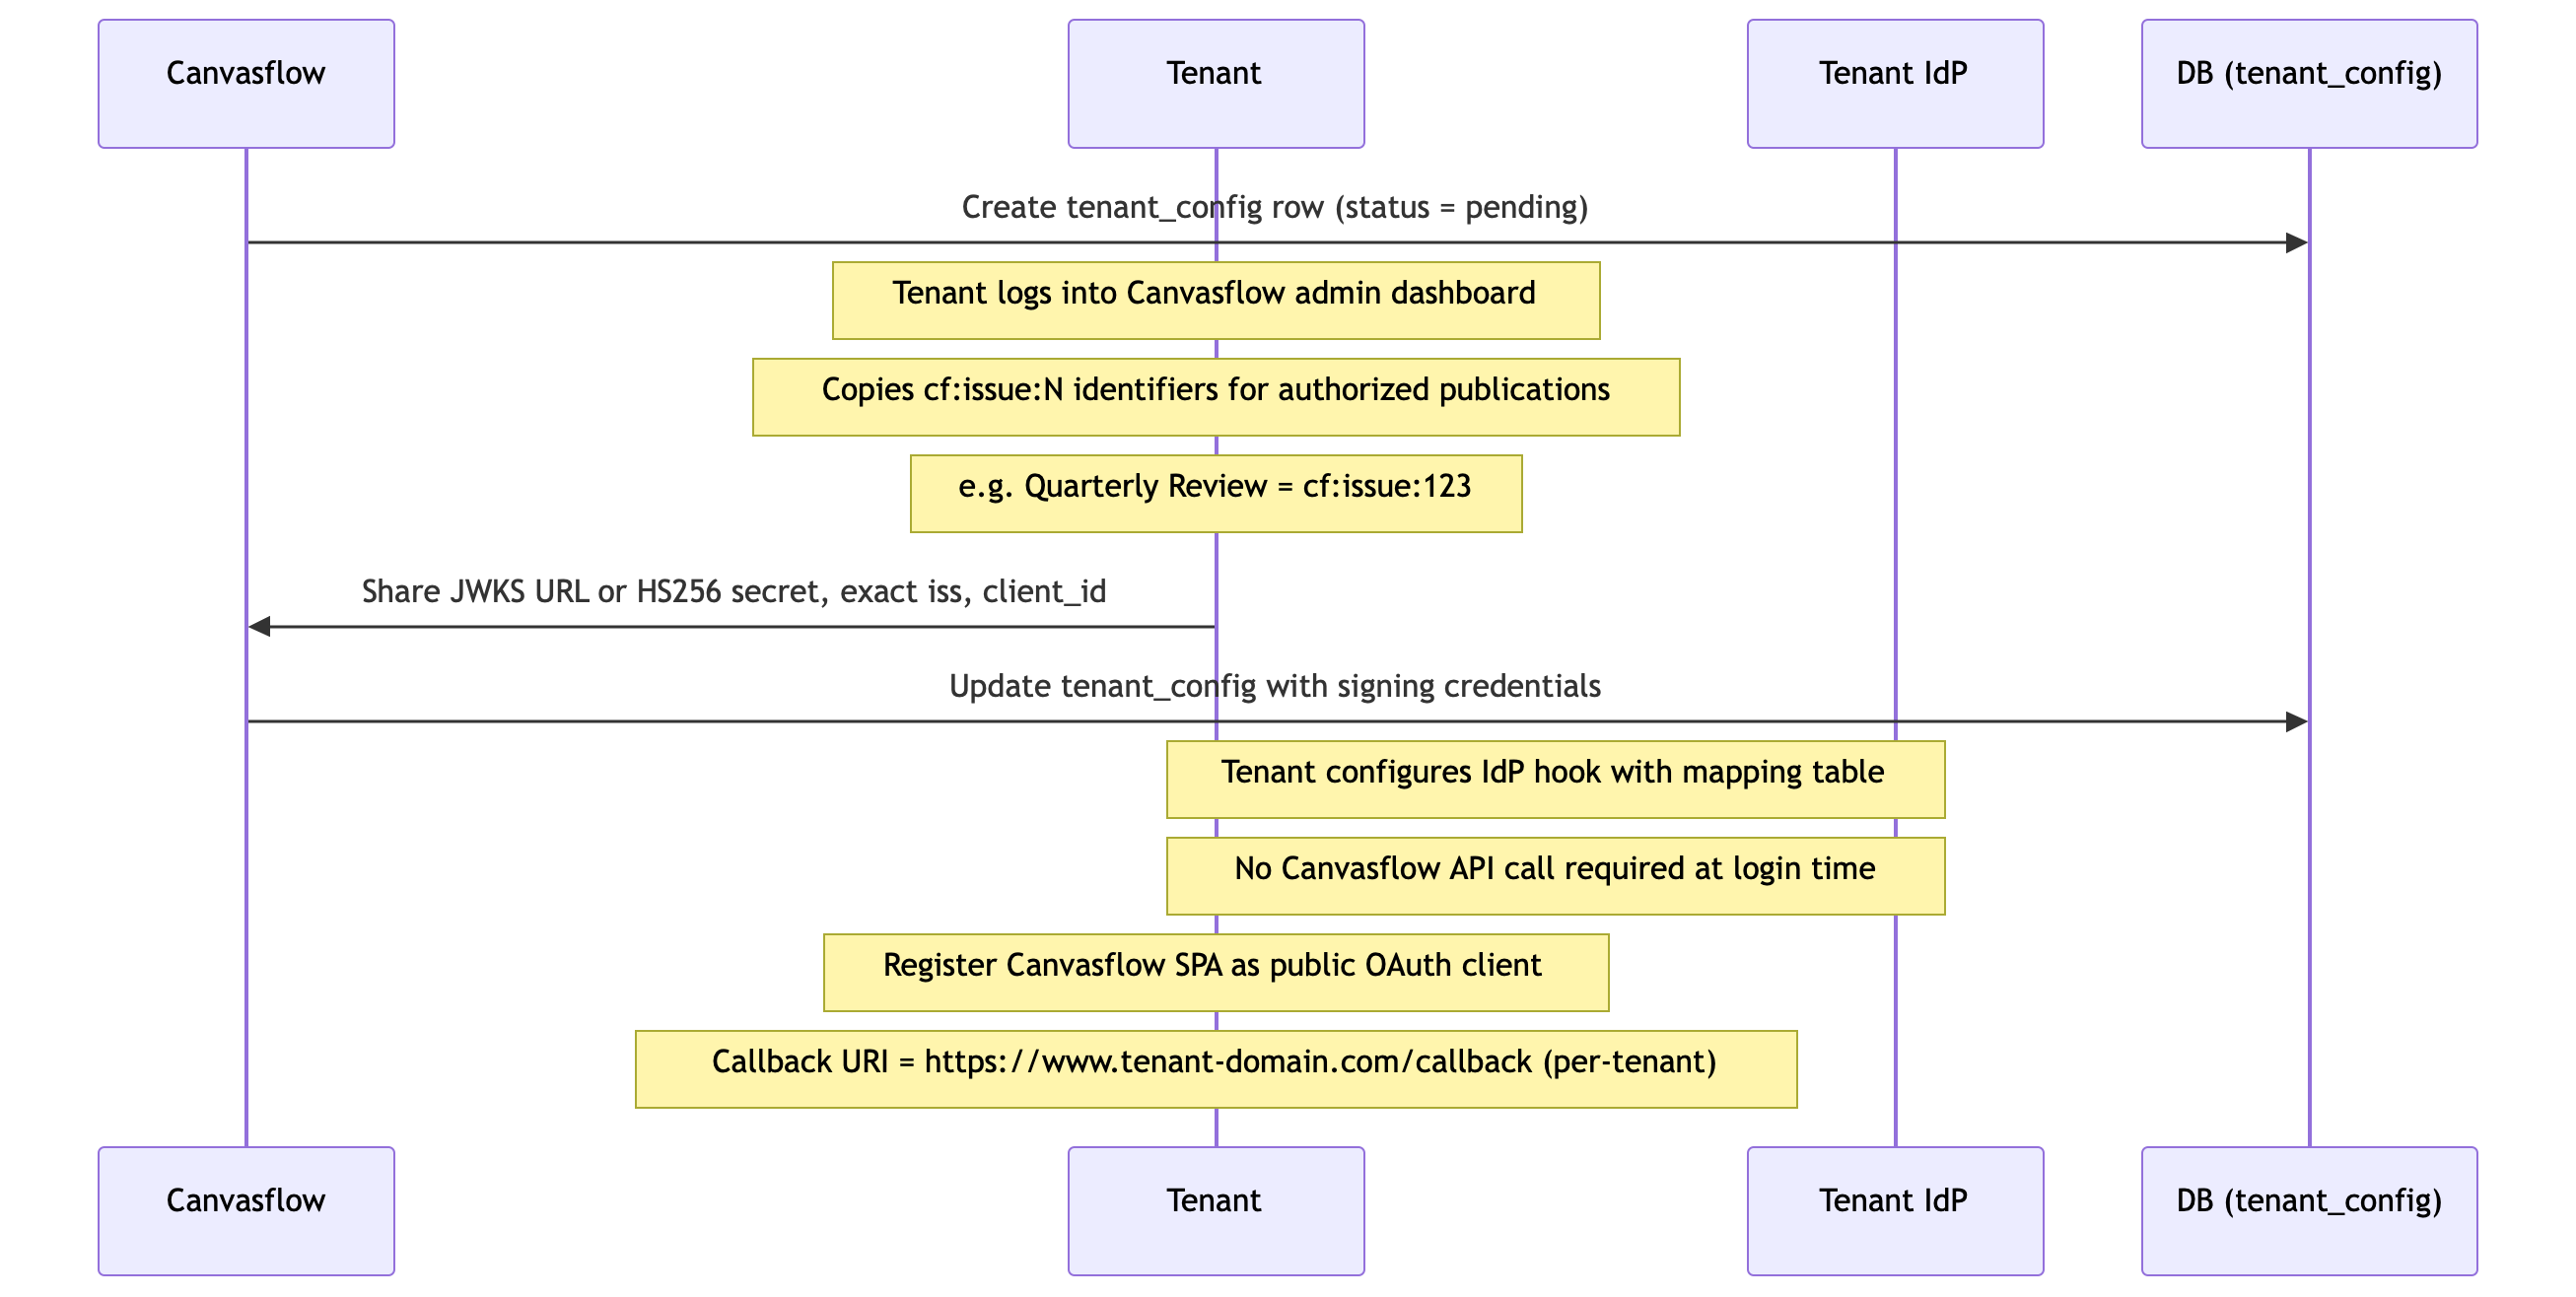
\includegraphics[width=1\textwidth]{on-boarding-diagram.png} % Injects and resizes the image
    \caption{Tenant Onboarding Sequence Diagram} % Caption for the image
    \label{fig:on-boarding} % Used for cross-referencing
\end{figure}

\pagebreak

\subsubsection{Authentication Time (Per-User Login)}

\begin{figure}[ht!]
    \centering % Centers the image horizontally
    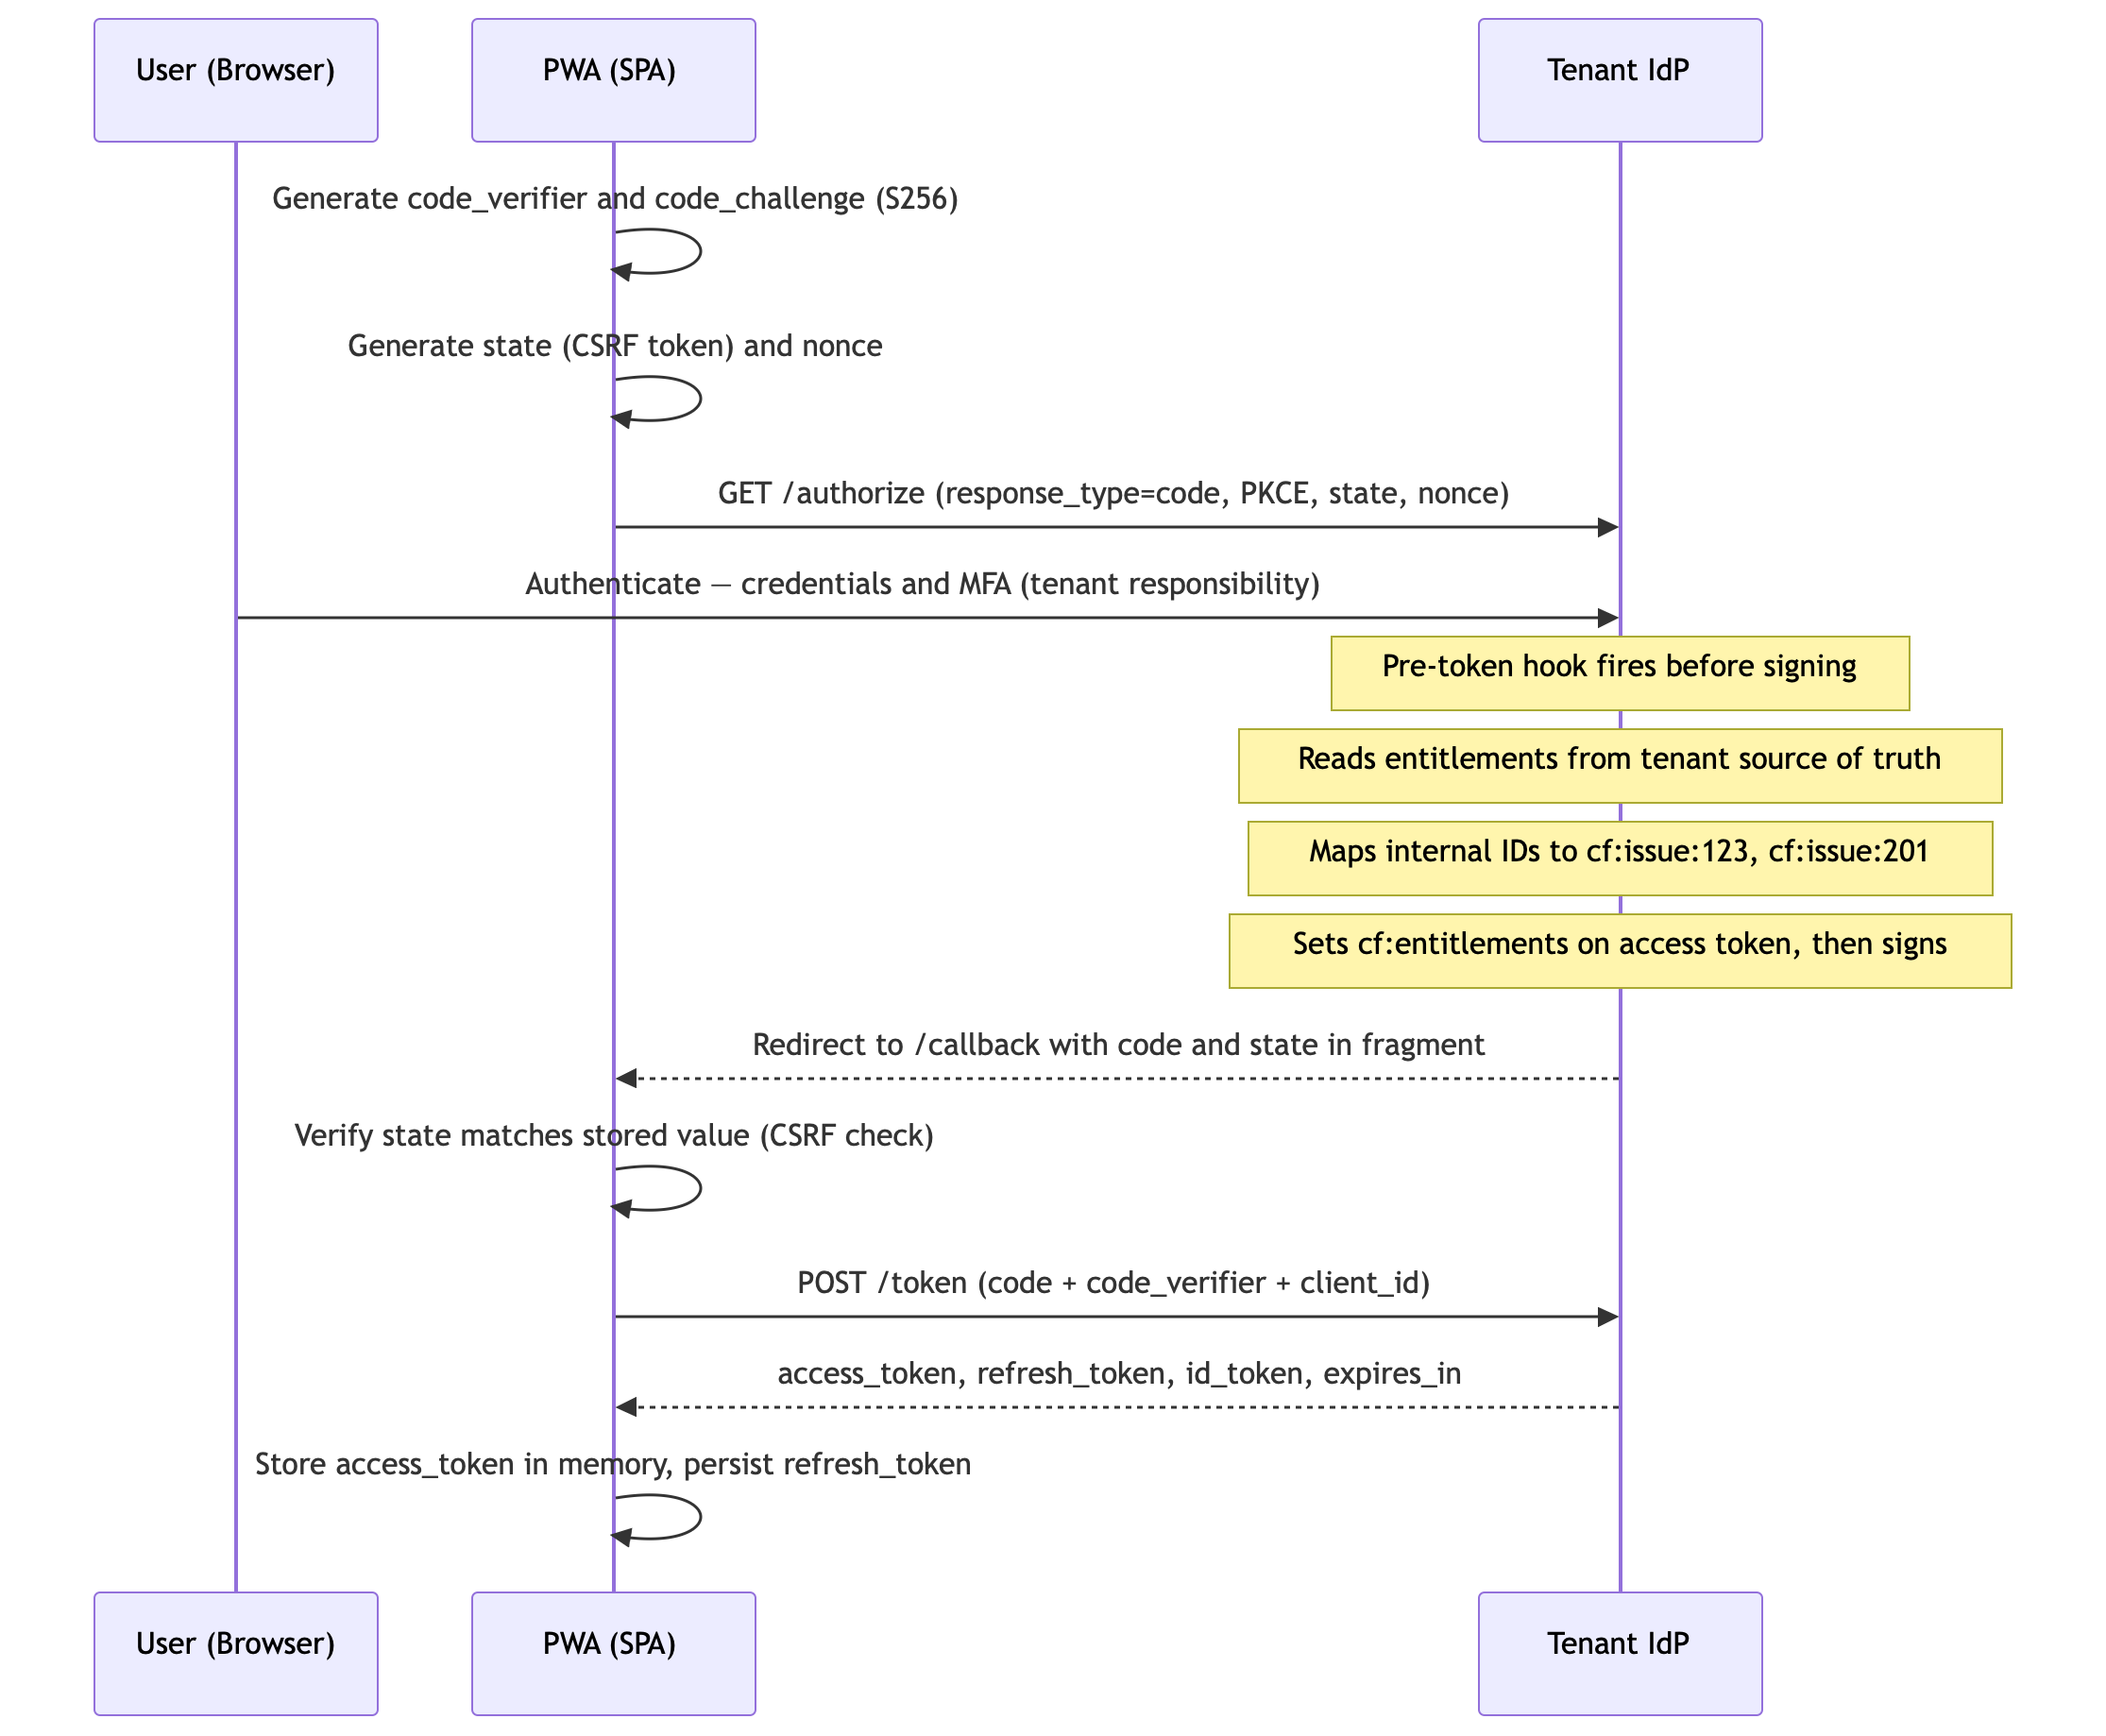
\includegraphics[width=1\textwidth]{authentication-diagram.png} % Injects and resizes the image
    \caption{Tenant Authentication Sequence Diagram} % Caption for the image
    \label{fig:authentication} % Used for cross-referencing
\end{figure}

\pagebreak

\subsubsection{Request Time (Per-API Call)}

\begin{figure}[ht!]
    \centering % Centers the image horizontally
    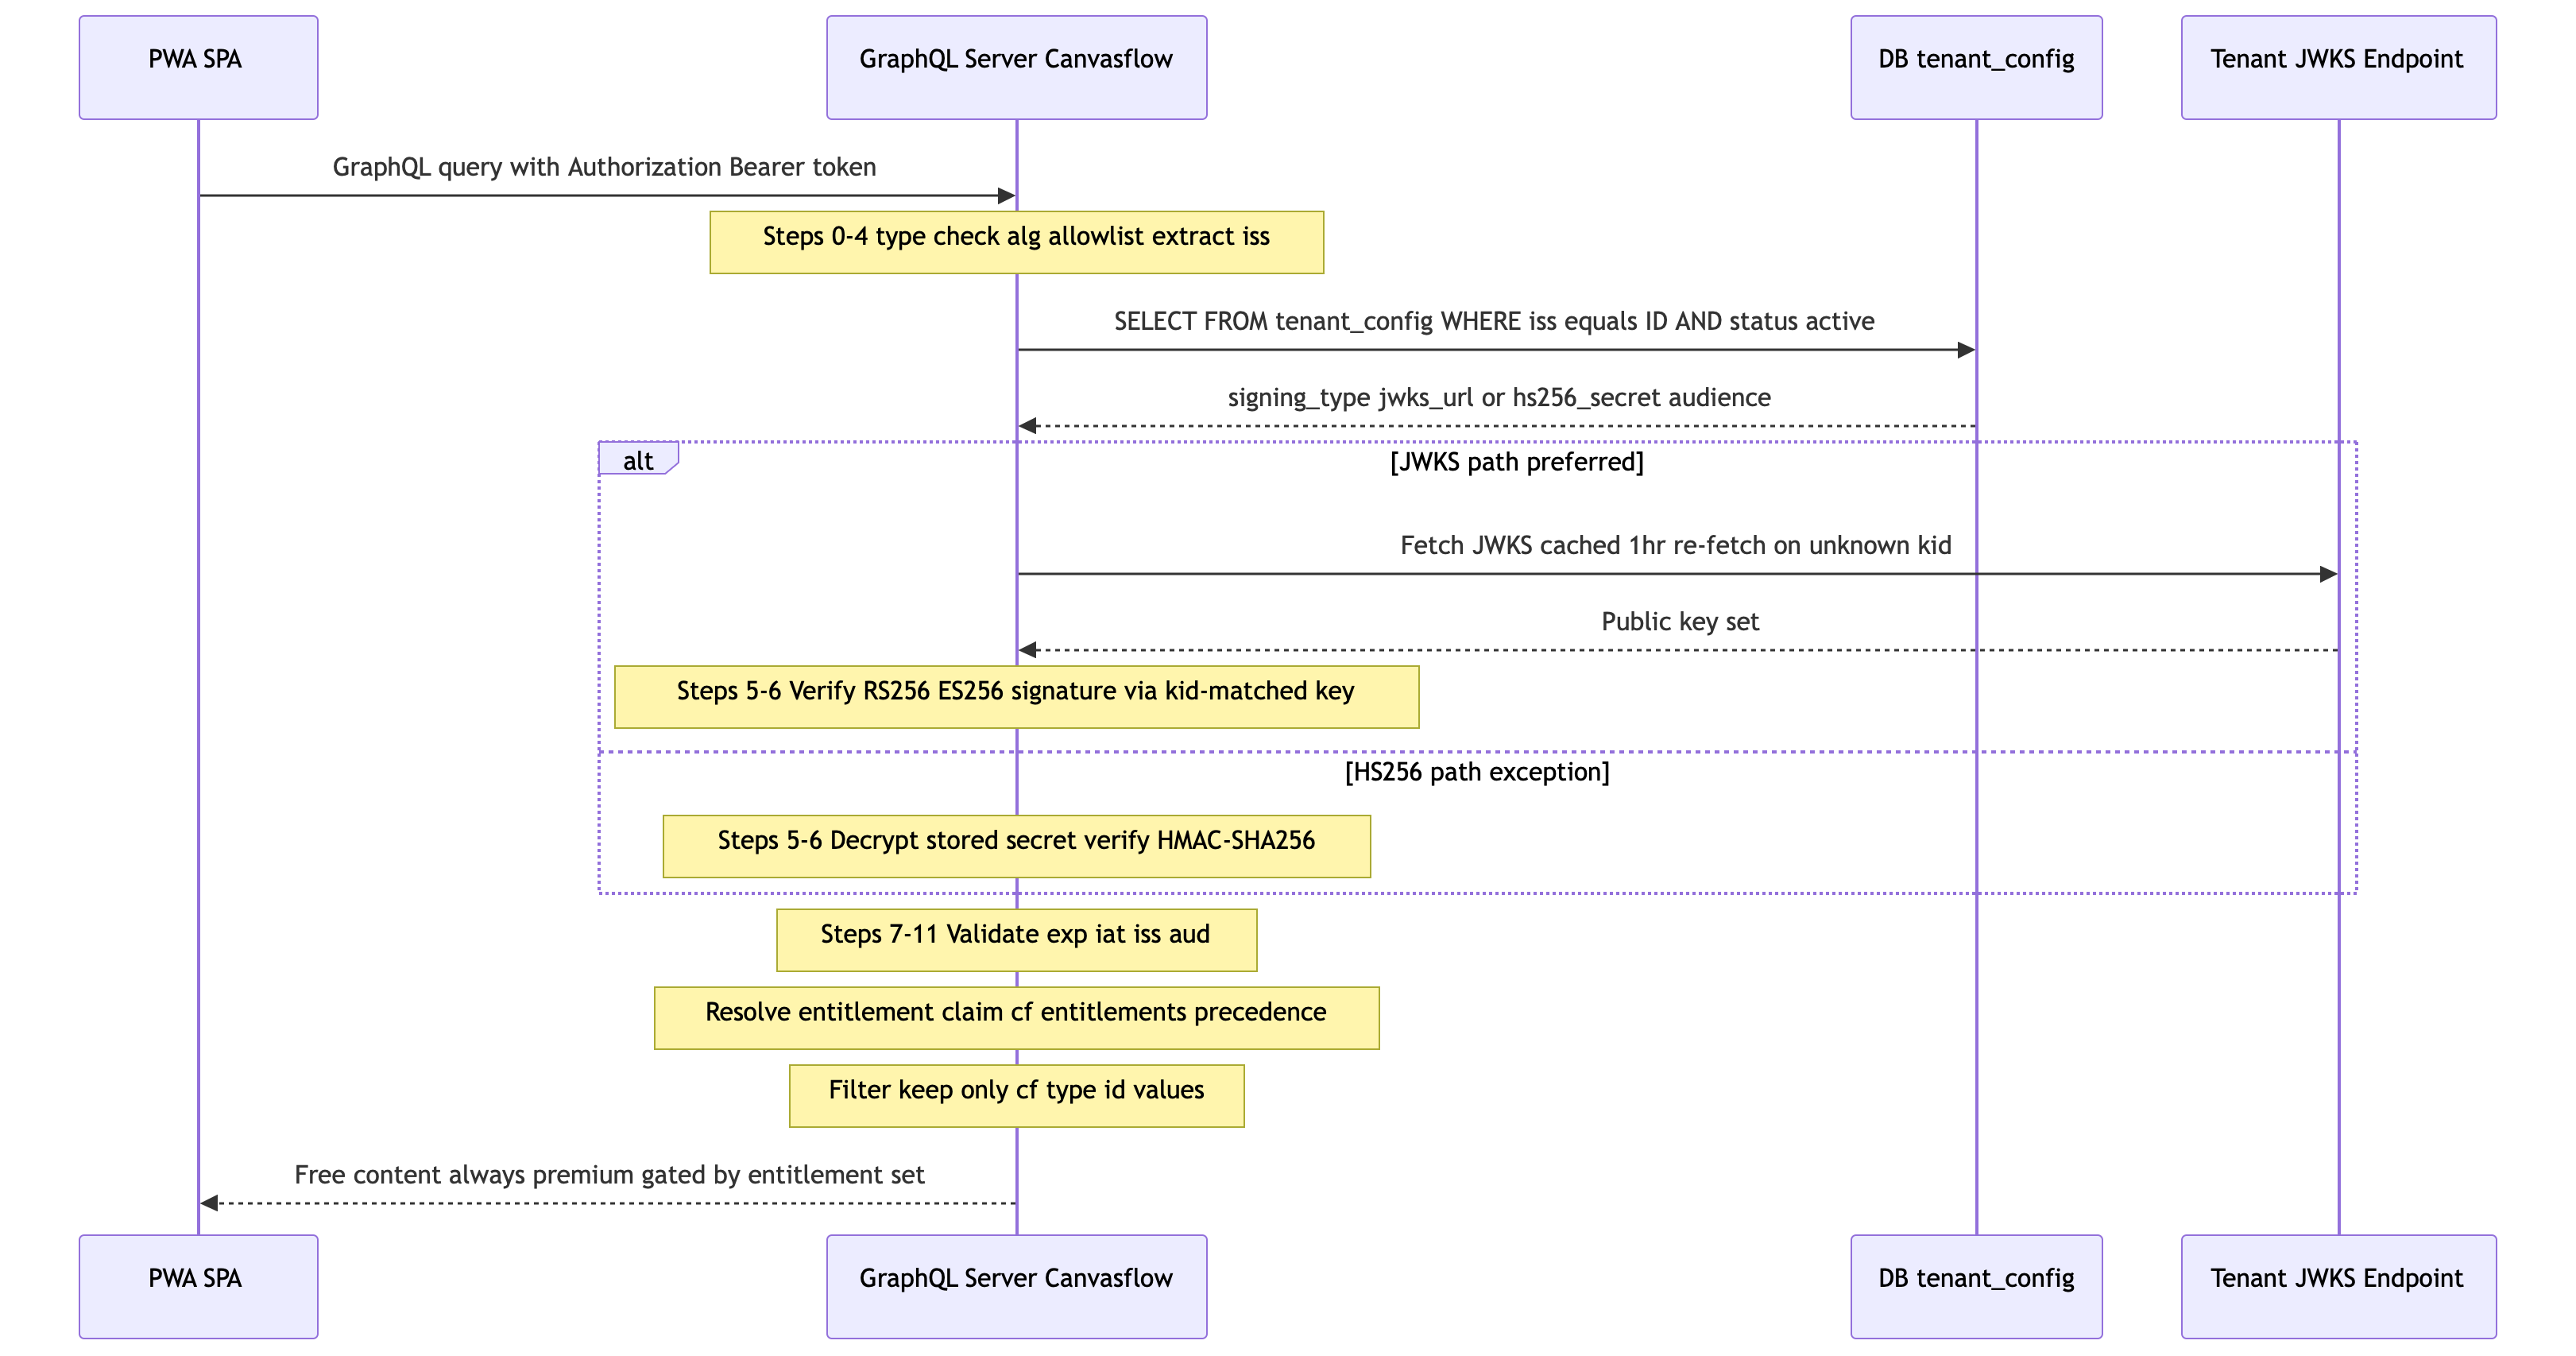
\includegraphics[width=1\textwidth]{request-diagram.png} % Injects and resizes the image
    \caption{Tenant Request Sequence Diagram} % Caption for the image
    \label{fig:request} % Used for cross-referencing
\end{figure}
\pagebreak
\section{Pre-requisites}

\textit{Normative language per \href{https://tools.ietf.org/html/rfc2119}{RFC~2119}.}

\subsection{Purpose}

This section defines the capabilities a tenant MUST possess before initiating
integration with Canvasflow. Meeting all pre-requisites is a mandatory precondition for
Phase~2 of the onboarding process (see \hyperref[sec:canvasflow-side-setup]{Canvasflow-Side Setup}). 
A tenant whose IdP does not satisfy all items in this section MUST resolve the gaps 
before proceeding; Canvasflow will not set \texttt{status = 'active'} for a tenant 
that cannot meet these requirements.


\subsection{Identity Provider Capabilities}

\subsubsection{OAuth 2.0 Authorization Code Flow}

The tenant's IdP MUST support the OAuth~2.0 Authorization Code flow as defined in
\href{https://datatracker.ietf.org/doc/html/rfc6749#section-4.1}{RFC~6749~\S4.1}. 
Specifically, the IdP MUST expose:

\begin{itemize}
  \item An authorization endpoint (\texttt{/authorize} or equivalent) capable of
    accepting \linebreak \texttt{response\_type=code} requests.
  \item A token endpoint (\texttt{/token} or equivalent) capable of exchanging
    authorization codes for access tokens, and of accepting
    \texttt{grant\_type=refresh\_token} for session renewal.
  \item A publicly accessible OIDC discovery document
    \linebreak(\texttt{/.well-known/openid-configuration}) or the ability to supply endpoint
    URLs directly to Canvasflow at onboarding.
\end{itemize}

\begin{quote}
  \textit{IdPs that support only the Implicit flow} (\href{https://datatracker.ietf.org/doc/html/rfc6749#section-4.2}{\textit{RFC~6749~\S4.2}})\textit{,
  the Resource Owner Password Credentials grant} (\href{https://datatracker.ietf.org/doc/html/rfc6749#section-4.3}{\textit{RFC~6749~\S4.3}})\textit{, 
  or the Client Credentials grant} (\href{https://datatracker.ietf.org/doc/html/rfc6749#section-4.4}{\textit{RFC~6749~\S4.4}}) \textit{do not satisfy this requirement. Those grants are not used in this
  integration.}
\end{quote}


\subsubsection{PKCE with S256 Challenge Method}



The tenant's IdP MUST support Proof Key for Code Exchange (PKCE) as defined in
\href{https://datatracker.ietf.org/doc/html/rfc7636}{RFC~7636} with the \texttt{S256} 
challenge method. The \texttt{plain} method MUST NOT be used. PKCE is required unconditionally, 
even if the tenant's IdP permits skipping it. This requirement exists for defense in depth: PKCE prevents both
authorization-code interception attacks and authorization-code injection attacks
(\href{https://datatracker.ietf.org/doc/html/rfc9700#section-4.4}{RFC~9700~\S4.4}). Tenants whose IdP marks PKCE as optional MUST configure their OAuth
client registration to enforce PKCE on the Canvasflow SPA client.

\pagebreak

\subsubsection{JWT Access Token Issuance}

The tenant's IdP MUST issue \textbf{JWT} (JSON Web Token, 
\href{https://datatracker.ietf.org/doc/html/rfc7519}{RFC~7519}) access 
tokens --- not opaque tokens. The Canvasflow Resource Server validates access 
tokens locally by verifying their cryptographic signature and claims; opaque 
tokens require introspection, which Canvasflow does not support.
\begin{quote}
  \textit{\textbf{Auth0 note (mandatory reading for Auth0 tenants):} Auth0 issues opaque access
  tokens by default when only an Application is registered. To obtain JWT access tokens,
  the tenant MUST register a separate \textbf{API} in the Auth0 dashboard and set its
  \texttt{identifier} (audience) to \texttt{canvasflow-api}. The Application must then
  have the API authorized; the PWA MUST include \texttt{audience=canvasflow-api} in every
  authorization request. An Application registration alone, without an accompanying API
  registration, will produce opaque access tokens that Canvasflow will reject.}
\end{quote}

\subsubsection{Pre-Token Hook Mechanism}

The tenant's IdP MUST provide a mechanism to execute custom logic server-side
immediately before an access token is signed. This hook is used to inject the
entitlement claim (\hyperref[sec:entitlement-mapping]{\S4}) into the access token payload. 
The hook MUST run on both initial login and on every token refresh.

The specific mechanism varies by IdP. Section \hyperref[sec:hook-configuration]{\S6} 
documents the correct mechanism for the four most common platforms. Tenants using 
an IdP not listed in \hyperref[sec:hook-configuration]{\S6} MUST confirm with 
Canvasflow that an equivalent mechanism exists before onboarding begins.

\subsubsection{Access Token Signing --- JWKS or HS256}

The tenant MUST use one of the two supported signing paths described 
in \hyperref[sec:signing-path-requirements]{\S5.2}:



\begin{itemize}
  \item \textbf{JWKS (preferred):} The IdP signs access tokens with RS256 or ES256, and
    publishes a JSON Web Key Set 
    (\href{https://datatracker.ietf.org/doc/html/rfc7517}{RFC~7517}) at a stable, 
    publicly accessible URL. This is the default path and is satisfied 
    automatically by AWS Cognito, Okta, Azure AD/Entra, and Auth0.

  \item \textbf{HS256 (exception):} The IdP signs access tokens with HMAC-SHA256 using
    a shared secret of at minimum 32~bytes (256~bits) of cryptographically random data.
    This path is an explicit exception reserved for custom or lightweight IdPs that
    cannot publish a JWKS endpoint. It MUST be approved by Canvasflow before use.
\end{itemize}

Both paths require that the \texttt{kid} (Key ID) header claim be present in every
issued token.

\subsubsection{Configurable Access Token Lifetime}

The tenant's IdP MUST be able to set the access token lifetime to a value no greater
than 3600~seconds (one hour). Longer lifetimes are prohibited 
(\hyperref[sec:required-payload-claims]{\S5.4}). The recommended lifetime is 
900--3600~seconds. A shorter lifetime reduces the revocation exposure window
(\hyperref[sec:revocation]{\S1.4}, Core Design Principle~3).

\subsection{Technical Personnel Requirement}

The tenant MUST designate a technical lead who has administrative access to the
tenant's IdP and who can:

\begin{enumerate}
  \item Register an OAuth~2.0 client application in the tenant's IdP.
  \item Implement and deploy the pre-token hook mechanism specific to their IdP (\hyperref[sec:hook-configuration]{\S6}).
  \item Obtain or confirm the signing credentials (JWKS URL or HS256 secret).
  \item Execute the full validation flow using the Canvasflow OAuth Validator tool
    (\url{https://oauth.canvasflow.work}) and produce evidence of all-green results for
    validation checks V1 through V5 (\hyperref[sec:tenant-side-setup]{Tenant-Side Setup}).
\end{enumerate}



No integration may proceed to go-live without a designated technical lead who has
completed the validation gate.

\subsection{Pre-Requisite Summary}

\begin{longtable}{@{}p{5cm}p{2cm}p{5cm}@{}}
\toprule
\textbf{Requirement} & \textbf{Mandatory?} & \textbf{Notes} \\
\midrule
\endhead
OAuth~2.0 Authorization Code flow (\href{https://datatracker.ietf.org/doc/html/rfc6749#section-4.1}{RFC~6749~\S4.1}) & MUST & Token endpoint must support refresh grant \\[4pt]
PKCE S256 (\href{https://datatracker.ietf.org/doc/html/rfc7636}{RFC~7636}) & MUST & Required even if IdP marks it optional \\[4pt]
JWT access token issuance & MUST & Auth0 requires separate API registration \\[4pt]
Pre-token hook on login AND refresh & MUST & Must inject entitlement claim into access token \\[4pt]
JWKS endpoint (RS256/ES256) & SHOULD & Preferred signing path \\[4pt]
HS256 shared secret ($\geq$~32 bytes) & MAY & Exception path; requires Canvasflow approval \\[4pt]
\texttt{kid} header in all issued tokens & MUST & Required for both signing paths \\[4pt]
Access token lifetime $\leq$ 3600 seconds & MUST & Hard limit; see \hyperref[sec:required-payload-claims]{\S5.4} \\[4pt]
Designated technical lead with IdP admin access & MUST & Required for validation gate \\[4pt]
Canvasflow OAuth Validator & MUST & Mandatory go-live gate \\
\bottomrule
\end{longtable}

\pagebreak
\section{Responsibilities}

\textit{Normative language per \href{https://tools.ietf.org/html/rfc2119}{RFC~2119}.}

\subsection{Purpose}

This section defines the responsibility boundary between the tenant (acting as the
OAuth~2.0 Authorization Server, 
\href{https://datatracker.ietf.org/doc/html/rfc6749#section-1.1}{RFC~6749~\S1.1}) 
and Canvasflow (acting as the OAuth~2.0 Resource Server, 
\href{https://datatracker.ietf.org/doc/html/rfc6749#section-1.1}{RFC~6749~\S1.1}). 
This matrix is the contractual heart of the integration. Any ambiguity about 
which party is responsible for a given function is resolved here.

\subsection{Tenant Responsibilities (Authorization Server)}

The tenant is the Authorization Server in the sense of 
\href{https://datatracker.ietf.org/doc/html/rfc6749#section-1.1}{RFC~6749~\S1.1}. 
The tenant is solely responsible for the following:

\subsubsection{User Authentication}

The tenant MUST perform all user authentication. This includes, but is not limited to:
credential verification (username and password, passkeys, certificates),
multi-factor authentication (MFA), social identity connections, and session initiation
and termination. Canvasflow has no visibility into the tenant's authentication mechanisms
and makes no assumptions about them.

\subsubsection{Authorization Decisions}

The tenant MUST make all authorization decisions. The determination of which users are
entitled to which Canvasflow resources is entirely the tenant's responsibility. These
decisions are encoded by the pre-token hook at login and refresh time and sealed into
the signed JWT. Canvasflow enforces these decisions; it does not make them.

\subsubsection{Entitlement Mapping}

The tenant MUST maintain the mapping between their internal product or entitlement
identifiers and Canvasflow resource identifiers. This mapping table lives inside the
tenant's own system --- in the IdP hook, a directory attribute, a hardcoded table, or a
lookup against the tenant's own database. The form is the tenant's choice; the output
MUST be an array of Canvasflow resource identifiers in \texttt{cf:<type>:<id>} format
(see \hyperref[sec:mandatory-value-format]{Entitlement Mapping \S4.2}).

This mapping MUST be re-evaluated on every login and every token refresh. The hook MUST
NOT copy the entitlement claim from a prior token; it MUST read from the tenant's live
source of truth on each invocation. This ensures that changes to entitlements propagate
within the revocation window ($\leq$ 3600~seconds, governed by the access token
\texttt{exp}).

\pagebreak

\subsubsection{Token Signing and Key Protection}

The tenant MUST sign all access tokens using a signing method that Canvasflow supports
(\hyperref[sec:signing-path-requirements]{\S5.2}). The tenant MUST protect its signing private keys (JWKS path) or shared secrets
(HS256 path). Canvasflow's guarantee that it cannot forge tokens on behalf of the tenant
depends on the tenant maintaining exclusive control of their private signing keys.

\subsubsection{Key Rotation}

\begin{itemize}
  \item \textbf{JWKS path:} The tenant MAY rotate keys at any time by publishing a new
    key pair under a new \texttt{kid} in their JWKS endpoint. The tenant MUST maintain
    the outgoing key in the JWKS for a minimum overlap window of one hour after the new
    key begins signing tokens. No coordination with Canvasflow is required for JWKS key
    rotation.

  \item \textbf{HS256 path:} The tenant MUST notify Canvasflow before rotating a shared
    secret. The tenant MUST provide the new secret via a secure channel and MUST
    maintain the outgoing secret as valid under its existing \texttt{kid} for a minimum
    of one hour after the new secret takes effect.
\end{itemize}

\subsubsection{Session Lifecycle}\label{sec:session-lifecycle}

The tenant is responsible for login, silent refresh, logout, and revocation of user
sessions. If the tenant needs to immediately cut off a user's access, the tenant MUST
revoke the user's refresh token in the IdP. The residual access window is bounded by
the access token \texttt{exp} ($\leq$ 3600~seconds). Canvasflow has no mechanism to
accelerate this revocation --- that is by design (see \hyperref[sec:out-of-scope]{\S1.4}).



\subsubsection{OAuth Client Registration}

The tenant MUST register the Canvasflow SPA as a public OAuth~2.0 client in their IdP
with the exact settings required in \hyperref[sec:tenant-side-setup]{\S9.3} (Step 2.2), including:

\begin{itemize}
  \item The exact callback URI: \texttt{https://www.<tenant-domain>/callback}
  \item Grant type: Authorization Code with PKCE (S256)
  \item Token endpoint authentication method: none (public client --- no client secret)
  \item Access token format: JWT with \texttt{typ: "at+jwt"} in the header
  \item Access token lifetime: $\leq$ 3600~seconds
\end{itemize}

\pagebreak

\subsection{Canvasflow Responsibilities (Resource Server)}\label{sec:canvasflow-responsibilities}

Canvasflow is the Resource Server in the sense of 
\href{https://datatracker.ietf.org/doc/html/rfc6749#section-1.1}{RFC~6749~\S1.1}. 
Canvasflow is responsible for the following:

\subsubsection{Token Validation on Every Request}

Canvasflow MUST validate the cryptographic signature and all required claims of every
access token received at the GraphQL API. 
% The complete, ordered validation sequence is defined in \texttt{spec\_appendix\_validation}. 
No request is authorized without passing the full sequence.

\subsubsection{Content Gating}

Canvasflow MUST gate GraphQL content strictly by the verified entitlement claim. Content
Canvasflow classifies as free MUST be returned to any bearer of a valid access token,
regardless of the entitlement set. Content Canvasflow classifies as premium MUST be
returned only when the matching \texttt{cf:<type>:<id>} value is present in the
effective entitlement set (see \hyperref[sec:claim-name-hierarchy]{Entitlement Mapping \S4.3}). 
Canvasflow MUST NOT apply any additional authorization logic beyond 
what the signed token encodes.

\subsubsection{JWKS Caching}

Canvasflow MUST fetch tenant JWKS documents server-side only and MUST cache them with a
TTL of one hour. An incoming token whose \texttt{kid} is not found in the cache triggers
an immediate JWKS re-fetch. Canvasflow MUST NOT serve stale JWKS keys when a re-fetch
fails; it MUST reject the token. JWKS key material is never exposed to clients.

\subsubsection{HS256 Secret Storage}

Canvasflow MUST store HS256 shared secrets encrypted at the application layer using
AES-256-GCM with a KMS-managed key. Secrets MUST never appear in logs or error
responses. Canvasflow MUST notify the affected tenant within 24~hours of any confirmed
or suspected compromise of a stored HS256 secret.

\subsubsection{Generic Error Responses}

Canvasflow MUST return generic 401 responses on all token validation failures. The
response MUST NOT reveal which validation step failed, which tenant was involved, or
which claim was absent or malformed. Detailed failure reasons are logged server-side and
correlated by \texttt{jti}. This policy is a security requirement; it prevents both
tenant enumeration and targeted token-forgery attacks.

\subsubsection{Resource ID Stability}

Canvasflow MUST NOT change the Canvasflow resource IDs (for example, \texttt{cf:issue:123})
assigned to a tenant after onboarding without prior written notice to the tenant's
designated technical lead. Resource ID stability is essential because these values are
hardcoded into the tenant's IdP hook mapping table.

\subsubsection{No Runtime Calls to the Tenant IdP}

Canvasflow MUST NOT call the tenant IdP at API request time for any purpose other than
a JWKS cache refresh triggered by an unknown \texttt{kid}. The tenant's IdP availability
MUST NOT be a dependency for serving already-issued access tokens.

\subsection{Justification}

The responsibility distribution above was designed to maximize system reliability and
minimize coupling.

\textbf{Stateless Resource Server.} By confining all authorization logic to the signed
JWT --- a decision sealed by the tenant's IdP before the token reaches Canvasflow --- the
Resource Server requires zero network calls in the hot path (JWKS key cache is warm).
This makes the Canvasflow API horizontally scalable without coordination and removes the
tenant's IdP from the availability dependency chain of every API request.

\textbf{Clean trust boundary.} The signed JWT is the sole interface between the two
systems. A tenant that rotates its signing keys, changes its user directory, or migrates
IdP platforms does so without touching the Canvasflow API layer, provided the output
token structure remains conformant with this specification.

\textbf{Bounded revocation window as a trade-off.} Delegating revocation to the tenant
and bounding the exposure window by $\texttt{exp} \leq 3600\,\mathrm{s}$ is a deliberate
design choice that preserves the stateless Resource Server model. This trade-off is
acceptable for content delivery and is documented here --- not hidden --- so that tenants
can evaluate it against their security requirements.
\pagebreak
\section{Entitlement Mapping}\label{sec:entitlement-mapping}

\textit{Normative language per \href{https://tools.ietf.org/html/rfc2119}{RFC~2119}.}

\subsection{How Mapping Works --- Tenant Responsibility}

The tenant is solely responsible for the mapping between their users' entitlements
(expressed in tenant-internal identifiers) and Canvasflow resource identifiers.

Canvasflow resource identifiers are stable and self-served. The Canvasflow administration 
dashboard lists every publication and content resource the tenant is authorized to access 
alongside its \texttt{cf:<type>:<id>} identifier (for example, \texttt{cf:issue:123}). 
The tenant's technical lead logs into the dashboard, locates the relevant publications, and 
copies the identifiers directly from the UI. No mapping document is delivered by 
Canvasflow; no API is called to retrieve identifiers. This retrieval is a one-time 
step performed during Phase 2 of onboarding 
(see \hyperref[sec:canvasflow-side-setup]{Client On-Boarding \S9.2}).


From that point forward, maintaining and executing the mapping is entirely the tenant's
responsibility. The tenant maintains the mapping table inside their own IdP hook. The
form of the mapping table is the tenant's choice --- a hardcoded table, a group attribute
lookup, a call to the tenant's internal directory, or any other mechanism. The required
output format is defined in \hyperref[sec:mandatory-value-format]{\S4.2} below.

At every login \textbf{and} every token refresh, the hook reads the authenticated user's
entitlements from the tenant's source of truth, maps them to Canvasflow resource
identifiers, and embeds the result in the \textbf{access token} before it is signed.
Canvasflow never sees tenant-internal product identifiers and never performs mapping
logic.

\textbf{No Canvasflow endpoint is called at login time.} The mapping is performed
entirely inside the tenant's IdP hook without contacting Canvasflow's servers.

\subsection{Mandatory Value Format: the \texttt{cf:} Prefix}\label{sec:mandatory-value-format}

Every entitlement value emitted by the tenant's hook into the access token MUST use the
format:

\begin{lstlisting}
cf:<type>:<id>
\end{lstlisting}

where \texttt{<type>} is the Canvasflow resource type (e.g., \texttt{issue}) and
\texttt{<id>} is the stable Canvasflow-assigned numeric or alphanumeric identifier for
that resource. Examples of conforming values:

\begin{lstlisting}
cf:issue:1111
cf:issue:201
cf:issue:123
\end{lstlisting}

\subsubsection{The Ignore Rule for Non-Prefixed Values}

The Canvasflow Resource Server applies a strict filter to every value in the resolved
entitlement array:

\begin{itemize}
  \item Values with the \texttt{cf:} prefix and the well-formed
    \texttt{cf:<type>:<id>} structure --- \textbf{accepted} and used for content gating.
  \item \textbf{Any value without the \texttt{cf:} prefix --- silently ignored.} It is
    dropped from the effective entitlement set. It does not cause the token to be
    rejected. It does not grant any access.
\end{itemize}

The effective entitlement set is computed as:

\begin{lstlisting}
effective_entitlements =
  resolved_claim_array
    .filter(v => typeof v === 'string' &&
            v.startsWith('cf:'))
\end{lstlisting}

\textbf{Example:} a claim value of
\texttt{["cf:issue:123",\ "product:789",\ "issue:201"]} yields an effective entitlement
set of \texttt{["cf:issue:123"]}. The values \texttt{product:789} (a tenant-internal
identifier without the prefix) and \texttt{issue:201} (missing the \texttt{cf:} prefix)
are both ignored and logged server-side correlated by \texttt{jti}.

\textbf{Why the prefix is required.} The \texttt{cf:} namespace makes entitlement values
self-describing and collision-proof. A raw tenant-internal identifier such as \texttt{456}
or \texttt{product:789} that leaks into the claim can never be mistaken for a Canvasflow
entitlement. The prefix also enables unambiguous filtering --- the Resource Server requires
no knowledge of any tenant's internal identifier scheme to apply the rule.

\textbf{Why the ignore-rather-than-reject behavior.} IdP hooks and shared claims
frequently carry values from other integrations or from incomplete mapping configurations.
Rejecting an entire token because one value in the array lacks the \texttt{cf:} prefix
would turn a partial misconfiguration into a full authentication outage for the affected
user. Silently ignoring non-prefixed values fails safe: unmapped or foreign values grant
nothing, and the user still authenticates. Server-side logging of ignored values
(correlated by \texttt{jti}) preserves the ability for Canvasflow support to assist the
tenant in identifying and correcting the misconfiguration.

\subsection{Claim Name Hierarchy and Precedence}\label{sec:claim-name-hierarchy}

The mapped entitlement array MAY be communicated under any one of three claim names.
When more than one is present in a single token, the Resource Server applies a strict
precedence rule.




\begin{table}[htbp]
\centering
\begin{tabularx}{\textwidth}{@{}clX@{}}
\toprule
\textbf{Precedence} & \textbf{Claim name} & \textbf{Why it exists} \\
\midrule
1 (highest) & \texttt{cf:entitlements} &
  Namespaced, collision-proof. Some IdPs --- notably Auth0 --- blocklist non-namespaced
  custom claims on access tokens. \texttt{cf:entitlements} is guaranteed to work on
  every IdP and is the RECOMMENDED claim name for all new integrations. \\[6pt]
2 & \texttt{resources} &
  Legacy claim name retained for backward compatibility with tenants already integrated
  against this name. \\[6pt]
3 (lowest) & \texttt{entitlements} &
  The IANA-registered claim name per 
  \href{https://tools.ietf.org/html/rfc9068\#section-2.2.3.1}{RFC~9068~\S2.2.3.1} and 
  \href{https://tools.ietf.org/html/rfc7643\#section-4.1.2}{RFC~7643~\S4.1.2} ---
  standards-preferred but usable only on IdPs that do not reserve or blocklist it. \\
\bottomrule
\end{tabularx}
\caption{Entitlement claim name precedence}
\end{table}

\textbf{Resolution rule (normative):} The Resource Server reads the first claim present
in precedence order and uses it exclusively. It does not merge arrays across multiple
claim names. If \texttt{cf:entitlements} is present, \texttt{resources} and
\texttt{entitlements} are ignored entirely, even if they contain additional values.

\begin{lstlisting}
if token.claims["cf:entitlements"] exists:
    resolved_claim_array =
      token.claims["cf:entitlements"]
else if token.claims["resources"] exists:
    resolved_claim_array =
      token.claims["resources"]
else if token.claims["entitlements"] exists:
    resolved_claim_array =
      token.claims["entitlements"]
else:
    resolved_claim_array = []   
\end{lstlisting}

\textbf{Why precedence is inverted from standards purity.} The namespaced claim
\texttt{cf:entitlements} takes priority over the standards-registered
\texttt{entitlements} because \emph{reliability beats purity}. A tenant who deliberately
sets \texttt{cf:entitlements} for Canvasflow has expressed clear intent --- whereas the
bare \texttt{entitlements} claim may have been populated by the IdP itself (as a standard
SCIM attribute) or by an unrelated integration. When both are present, the namespaced
claim is the authoritative signal of what the tenant intended for this integration.

\textbf{Recommendation.} All new integrations SHOULD use \texttt{cf:entitlements}.
Existing integrations using \texttt{resources} or \texttt{entitlements} are supported
but SHOULD migrate to \texttt{cf:entitlements} at their next major hook update. Auth0
tenants MUST use \texttt{cf:entitlements} --- no other option is available (see
\hyperref[sec:per-idp-implementation]{Per-IdP Implementation Table \S6.2}).

\pagebreak

\subsection{Empty, Absent, and All-Ignored Claims: the Free-Content Baseline}\label{sec:free-content-baseline}

The following three states all resolve to the same effective condition:

\begin{table}[htbp]
\centering
\begin{tabularx}{\textwidth}{@{ }p{1.3cm}Xp{3cm}@{}}
\toprule
\textbf{State} & \textbf{Cause} & \textbf{Effective entitlement set} \\
\midrule
Empty array & \texttt{"cf:entitlements":[]} emitted by hook & \texttt{[]} \\[4pt]
Absent claim & None of the three claim names present & \texttt{[]} (logged as possible misconfiguration) \\[4pt]
All-ignored array & All values present but none carry \texttt{cf:} prefix & \texttt{[]} (logged as likely mapping misconfiguration) \\
\bottomrule
\end{tabularx}
\caption{Free-content baseline: three equivalent states}
\end{table}

In all three cases: \textbf{the user authenticates successfully and is entitled to free
content only.} Authentication does not fail. Content Canvasflow classifies as free is
served. Content Canvasflow classifies as premium is withheld. This is the semantic model
--- not an error condition.

Entitlements gate \emph{premium} content. Free content requires only a valid, verified
access token; entitlement values are not consulted.

\subsubsection{Consequences}

The following specific behaviors MUST be understood by tenant implementors:

\begin{itemize}
  \item \textbf{An empty array is a valid, intentional configuration.} A registered user
    on a free tier SHOULD have the hook emit \texttt{"cf:entitlements": []} explicitly.
    Explicit presence distinguishes ``free-tier user with correctly-configured hook'' from
    ``misconfigured hook with missing claim'' in server-side debugging.

  \item \textbf{An absent claim is tolerated} --- the behavior is identical to an empty
    array --- but Canvasflow MUST log a warning server-side (correlated by \texttt{jti})
    flagging the absence as a possible hook misconfiguration. An absent claim means
    Canvasflow cannot distinguish a deliberate free-tier configuration from a broken hook.

  \item \textbf{A present-but-non-array value MUST cause token rejection (401).} If the
    resolved claim name is present but its value is not a JSON array (e.g., it is a
    string, number, or object), the token is malformed and MUST be rejected. A malformed
    claim is a broken token, not a free-tier user.

  \item \textbf{An all-ignored array} (values present, none carry the \texttt{cf:}
    prefix) results in free content only. The non-prefixed values are logged server-side
    (correlated by \texttt{jti}) as a likely mapping misconfiguration, but the token is
    not rejected.
\end{itemize}

\pagebreak

\subsection{Why Mapping Happens at Auth Time in the Hook}

Mapping is executed in the IdP hook at authentication and refresh time rather than in
the Canvasflow GraphQL server at request time. The justification is as follows:

\textbf{Performance.} The hook is called once per login or refresh, not on every API
request. Executing entitlement mapping inside the GraphQL resolver would add a
cross-system lookup to every query, multiplying the latency cost proportionally with
API usage volume.

\textbf{Cryptographic integrity.} The result of the hook's mapping is sealed inside the
JWT's signature before the token leaves the tenant's IdP. Any post-issuance tampering
with the entitlement claim invalidates the signature. The Resource Server does not need
to trust any runtime claim about entitlements --- it trusts only the signed token.

\textbf{Resource Server purity.} The Canvasflow GraphQL server has no knowledge of any
tenant's internal product identifiers. The mapping result arrives as Canvasflow resource
identifiers (\texttt{cf:issue:123}) already resolved; the server applies a set membership
check --- not a mapping operation. This keeps the Resource Server stateless.

\textbf{Trade-off.} Entitlement changes take effect at the user's next login or refresh.
Existing tokens are valid until their \texttt{exp}. The maximum staleness window is
bounded by $\texttt{exp} \le 3600$ seconds. This trade-off is acceptable for
content delivery; if a tenant requires immediate revocation, the mitigation is to revoke
the user's refresh token in the IdP, which prevents new access tokens from being issued
and limits the exposure window to the remaining lifetime of the current access token.

\subsection{Why Tenant-Managed Rather Than a Canvasflow Mapping Endpoint}

An alternative design --- where Canvasflow provides an endpoint that the IdP hook calls
at login time to perform the mapping --- was considered and rejected:

\begin{itemize}
  \item It would add a runtime dependency on Canvasflow's availability to every user
    login. A Canvasflow outage would prevent tenants from logging in.
  \item It would require the IdP hook to hold a Canvasflow API key, creating a
    secret-management obligation on the tenant side.
  \item The mapping logic lives closest to the data it maps. The tenant knows their own
    product identifiers and their own users' entitlements; Canvasflow does not.
  \item The design would require Canvasflow to build, operate, and secure a
    tenant-facing mapping API --- increasing the attack surface of the Canvasflow
    platform.
\end{itemize}

A Canvasflow-managed mapping endpoint is a candidate feature for a future version when
tenant mapping volume or complexity grows beyond what can be maintained in an IdP hook.

\pagebreak

\section{Token Requirements}\label{sec:token-requirements}

\textit{Normative language per \href{https://tools.ietf.org/html/rfc2119}{RFC~2119}.}

\subsection{Overview}


This section defines the complete structural requirements for JWT access tokens issued
by a tenant's IdP and presented to the Canvasflow GraphQL API. A token MUST satisfy
every requirement in \hyperref[sec:signing-path-requirements]{\S5.2}\ through 
\hyperref[sec:prohibited]{\S5.5} to be accepted. 
% The normative validation sequence the Resource Server applies is defined in \texttt{spec\_appendix\_validation}.

All example values in this section use: \linebreak
\texttt{iss = https://login.tenant.com}, 
\texttt{aud = canvasflow-api}, and entitlement values in the mandatory
\texttt{cf:<type>:<id>} format.

\subsection{Signing Path Requirements}\label{sec:signing-path-requirements}

Canvasflow supports two signing paths. The choice MUST be made at onboarding and
recorded in the tenant configuration. The two paths are not interchangeable after go-live
without a coordinated migration.

\subsubsection{Path A --- JWKS Endpoint (Preferred)}\label{sec:jwks-endpoint}

The tenant's IdP signs access tokens using an asymmetric algorithm (RS256 or ES256) and
publishes the corresponding public keys at a stable JSON Web Key Set (JWKS) endpoint per
\href{https://datatracker.ietf.org/doc/html/rfc7517}{RFC~7517}.

\textbf{Requirements:}

\begin{itemize}
  \item Algorithm MUST be RS256 or ES256 (RFC~7518~\href{https://datatracker.ietf.org/doc/html/rfc7518\#section-3.3}{\S3.3} and \href{https://datatracker.ietf.org/doc/html/rfc7518\#section-3.4}{\S3.4}).
  \item RSA keys MUST be at minimum 2048~bits in length.
  \item EC keys MUST use the P-256 curve.
  \item The \texttt{kid} header claim MUST be present in every issued token and MUST
    match a key in the JWKS endpoint.
  \item The JWKS URL MUST be publicly accessible (no authentication required to fetch it).
  \item The tenant MUST communicate the exact JWKS URL to Canvasflow at onboarding.
  \item \textbf{Key rotation:} the tenant MUST publish the new key alongside the outgoing
    key for a minimum overlap window of one hour before removing the outgoing key.
    Canvasflow resolves \texttt{kid} dynamically against a one-hour cache; an unknown
    \texttt{kid} triggers an immediate re-fetch. The one-hour overlap window is required
    to prevent transient 401 errors during rotation.
\end{itemize}

\begin{table}[htbp]
\centering
\begin{tabularx}{\textwidth}{@{}lX@{}}
\toprule
\textbf{IdP} & \textbf{JWKS URL format} \\
\midrule
AWS Cognito      & {\scriptsize\texttt{https://cognito-idp.<region>.amazonaws.com/<pool-id>/.well-known/jwks.json}} \\[4pt]
Okta             & {\scriptsize\texttt{https://<tenant>.okta.com/oauth2/v1/keys}} \\[4pt]
Azure AD / Entra & {\scriptsize\texttt{https://login.microsoftonline.com/<tenant-id>/discovery/v2.0/keys}} \\[4pt]
Auth0            & {\scriptsize\texttt{https://<tenant>.auth0.com/.well-known/jwks.json}} \\[4pt]
\bottomrule
\end{tabularx}
\caption{Well-known JWKS endpoint formats for major IdPs}
\end{table}

\pagebreak

\subsubsection{Path B --- HS256 Shared Secret (Exception)}

The tenant's IdP signs access tokens using HMAC-SHA256 with a shared secret that both
the tenant and Canvasflow hold. This path is an explicit exception reserved for custom
or lightweight IdPs that cannot publish a JWKS endpoint. It MUST be explicitly approved
and documented by Canvasflow before use.

\textbf{Requirements:}

\begin{itemize}
  \item Algorithm MUST be HS256.
  \item The shared secret MUST be at minimum 32~bytes (256~bits) of cryptographically
    random data. A secret shorter than 32~bytes MUST be rejected.
  \item The \texttt{kid} header claim MUST be present in every issued token and MUST
    match a known secret version in Canvasflow's configuration. This supports rotation.
  \item The tenant MUST share the secret with Canvasflow via a secure channel --- never
    via unencrypted email.
  \item \textbf{Key rotation:} the tenant MUST notify Canvasflow before rotating the
    secret, provide the new secret via a secure channel, and maintain the outgoing secret
    as valid under its current \texttt{kid} for at minimum one hour after the new secret
    begins signing tokens.
\end{itemize}

\textbf{Justification for JWKS over HS256.} The following four considerations make JWKS
the strongly preferred path:

\begin{enumerate}
  \item \textbf{Asymmetry of forgery risk.} With JWKS (RS256/ES256), Canvasflow holds
    only the tenant's public key. A total compromise of Canvasflow's infrastructure gives
    an attacker no ability to forge valid tokens for any JWKS tenant. With HS256, the
    shared secret is simultaneously a verification key and a signing key: a breach of
    Canvasflow's secret store allows an attacker to forge arbitrary valid tokens for
    every HS256 tenant.

  \item \textbf{Self-service key rotation.} A JWKS tenant rotates keys by publishing a
    new key pair under a new \texttt{kid} alongside the outgoing key. Canvasflow
    resolves \texttt{kid} dynamically; rotation requires zero coordination with Canvasflow
    and incurs zero downtime. HS256 rotation requires out-of-band secret exchange,
    coordinated timing, and a Canvasflow-side configuration update on every rotation.

  \item \textbf{No secret-handling liability.} A JWKS URL is public information. Every
    HS256 secret Canvasflow holds is standing security liability (\hyperref[sec:canvasflow-guarantees]{\S11}).

  \item \textbf{Zero marginal cost for enterprise IdPs.} AWS Cognito, Okta, Azure AD /
    Entra, and Auth0 all publish JWKS endpoints by default.
\end{enumerate}

\textbf{Conclusion:} JWKS is the default. HS256 is an explicit, documented exception
accepted as a trade of security posture for reduced onboarding friction, available only
when the tenant has confirmed that a JWKS endpoint is not achievable.

\subsection{Required Header Claims}

The following claims MUST be present in the JWT header of every access token:



\subsubsection{\texttt{typ} --- Token Type (RFC~9068~\S2.1)}\label{sec:token-type}

The \texttt{typ} header MUST be set to exactly \texttt{"at+jwt"} or
\texttt{"application/at+jwt"}.

\textbf{Rationale.} This is the primary defense against token confusion attacks. An
attacker who obtains an OIDC ID token --- which is signed by the same key as the access
token and carries valid \texttt{iss}, \texttt{sub}, and \texttt{aud} claims --- could
present it to the GraphQL API. Without \texttt{typ} validation, the signature would
verify and many claim checks would pass. The \texttt{typ: "at+jwt"} header is the
mechanism defined by 
\href{https://datatracker.ietf.org/doc/html/rfc9068#section-2.1}{RFC~9068~\S2.1} 
specifically to defeat this class of attack. The \texttt{typ} check MUST be 
performed before any payload claim is inspected.



\textbf{Cognito exception.} AWS Cognito emits \texttt{typ: "JWT"} and
\texttt{token\_use: "access"} instead of \texttt{typ: "at+jwt"}. This is a documented
non-compliance with \href{https://datatracker.ietf.org/doc/html/rfc9068}{RFC~9068}. Canvasflow accommodates this via a per-tenant
\texttt{typ\_strict} configuration flag. When a tenant's configuration carries
\texttt{typ\_strict = false} (set at onboarding for Cognito tenants), the Resource
Server accepts \texttt{typ: "JWT"} and enforces \texttt{token\_use == "access"} as a
substitute check. Tenants using Cognito MUST declare this at onboarding. All other
tenants MUST produce \texttt{typ: "at+jwt"}.

\subsubsection{\texttt{alg} --- Signing Algorithm (RFC~8725~\S3.1)}

The \texttt{alg} header MUST be one of: \texttt{"RS256"}, \texttt{"ES256"},
\texttt{"HS256"}.



The value \texttt{"none"} MUST be rejected unconditionally regardless of any other token
properties (\href{https://datatracker.ietf.org/doc/html/rfc8725#section-3.1}{RFC~8725~\S3.1}). 
The Resource Server MUST validate the \texttt{alg} header against the allowlist 
before performing any verification and MUST NOT use an algorithm
value taken from the token without this check.

\subsubsection{\texttt{kid} --- Key Identifier}

The \texttt{kid} header MUST be present. For JWKS tenants, it selects the public key
from the JWKS endpoint. For HS256 tenants, it selects the secret version from the stored
secret set. A token without \texttt{kid} MUST be rejected.

\pagebreak

\subsection{Required Payload Claims}\label{sec:required-payload-claims}

The following claims MUST be present in the JWT payload of every access token:

\begin{longtable}{@{}lp{1.5cm}p{8cm}@{}}
\toprule
\textbf{Claim} & \textbf{Type} & \textbf{Requirement} \\
\midrule
\endhead
\texttt{iss} & string &
  Tenant issuer URL. MUST exactly match the value registered in \texttt{tenant\_config}.
  Trailing slash is significant: \texttt{https://login.tenant.com} $\neq$
  \texttt{https://login.tenant.com/}. \\[6pt]
\texttt{sub} & string &
  Stable, opaque user identifier assigned by the tenant's IdP. MUST NOT be the user's
  email address (\href{https://datatracker.ietf.org/doc/html/rfc9068\#section-2.2}{RFC~9068~\S2.2}). 
  The \texttt{sub} value MUST remain stable across
  sessions for the same user. \\[6pt]
\texttt{aud} & string or array &
  MUST contain \texttt{"canvasflow-api"}. MAY be an array of strings
  (\href{https://datatracker.ietf.org/doc/html/rfc7519\#section-4.1.3}{RFC~7519~\S4.1.3} 
  permits arrays). Validation passes if \texttt{"canvasflow-api"} is
  \emph{present} in the \texttt{aud} value --- it need not be the only value. \\[6pt]
\texttt{iat} & number &
  Unix timestamp of issuance (seconds since epoch). MUST NOT be more than 60~seconds in
  the future (clock skew tolerance). \\[6pt]
\texttt{exp} & number &
  Unix timestamp of expiry (seconds since epoch). MUST be greater than the current time
  (with $\leq$~60 seconds clock skew tolerance). The difference
  $\texttt{exp} - \texttt{iat}$ MUST NOT exceed 3600~seconds. \\[6pt]
\texttt{jti} & string &
  Unique token identifier. A UUID is RECOMMENDED (\href{https://datatracker.ietf.org/doc/html/rfc4122}{RFC~4122}). 
  Used for server-side log correlation; NOT used for revocation (by design --- 
  see \hyperref[sec:canvasflow-responsibilities]{\S3.3} and 
  \hyperref[sec:out-of-scope]{\S1.4}). \\[6pt]
Entitlement claim & array &
  One of \texttt{cf:entitlements}, \texttt{resources}, or \texttt{entitlements} per the
  precedence rules in \hyperref[sec:claim-name-hierarchy]{\S4.3}. The resolved value MUST
  be a JSON array of strings. An empty array is valid. \\
\bottomrule
\end{longtable}

\begin{quote}
  \textbf{Auth0 \texttt{aud} note.} When the \texttt{openid} scope is requested, Auth0
  includes both \linebreak \texttt{"canvasflow-api"} and the Auth0 \texttt{/userinfo} URL in the
  \texttt{aud} claim as an array. This is fully compliant with 
  \href{https://datatracker.ietf.org/doc/html/rfc7519\#section-4.1.3}{RFC~7519~\S4.1.3}.
  Canvasflow's validation passes as long as \texttt{"canvasflow-api"} is present in the
  array.
\end{quote}

\pagebreak

\subsection{Prohibited}\label{sec:prohibited}

The following MUST NOT appear in any conforming access token:





\begin{longtable}{@{}p{5.5cm}p{9cm}@{}}
\toprule
\textbf{Prohibited} & \textbf{Reason} \\
\midrule
\endhead
\texttt{alg: "none"} &
  Eliminates signature verification entirely; unconditional rejection per 
  \href{https://datatracker.ietf.org/doc/html/rfc8725\#section-3.1}{RFC~8725~\S3.1}. \\[6pt]
\texttt{typ} absent, \texttt{typ: "JWT"} (except Cognito with \texttt{typ\_strict=false}), \texttt{typ: "id\_token+jwt"}, or any other non-compliant \texttt{typ} &
  Enables token confusion attacks (\href{https://datatracker.ietf.org/doc/html/rfc9068\#section-2.1}{RFC~9068~\S2.1}). \\[6pt]
PII in the access token payload (name, email, physical address, phone number) &
  Access tokens traverse multiple systems; PII creates unnecessary exposure risk. \\[6pt]
RSA key shorter than 2048~bits &
  Computationally feasible to break; below the minimum security level for RS256
  (\href{https://datatracker.ietf.org/doc/html/rfc7518\#section-3.3}{RFC~7518~\S3.3}). \\[6pt]
$\texttt{exp} - \texttt{iat}$ greater than 3600~seconds &
  Exceeds the maximum allowed revocation window (\hyperref[sec:revocation]{\S1.4}, Core Design Principle~3). \\[6pt]
Entitlement claim placed in the ID token instead of the access token &
  The ID token is consumed by the SPA and never sent to the API; the claim would be
  silently absent from the Resource Server's perspective. \\[6pt]
Email address as \texttt{sub} &
  Email addresses are mutable; \texttt{sub} must be a stable, opaque identifier
  (\href{https://datatracker.ietf.org/doc/html/rfc9068\#section-2.2}{RFC~9068~\S2.2}). \\
\bottomrule
\end{longtable}

\pagebreak

\subsection{Conforming Token Example}

The following example shows a fully conforming JWT access token using the JWKS (RS256)
signing path and the recommended \texttt{cf:entitlements} claim name.
\linebreak\linebreak
\textbf{Header:}

\begin{lstlisting}[language=json]
{
  "typ": "at+jwt",
  "alg": "RS256",
  "kid": "tenant-key-v3"
}
\end{lstlisting}

\textbf{Payload:}

\begin{lstlisting}[language=json]
{
  "iss": "https://login.tenant.com",
  "sub": "usr_7f3a9c1d-opaque",
  "aud": "canvasflow-api",
  "iat": 1720224000,
  "exp": 1720227600,
  "jti": "a8f3c1d2-9e4b-4f7a-b6c5-1234567890ab",
  "client_id": "canvasflow-pwa",
  "cf:entitlements": ["cf:issue:123", "cf:issue:201"]
}
\end{lstlisting}



Notes on this example:
\begin{itemize}
  \item $\texttt{exp} - \texttt{iat} = 3600$ seconds --- the maximum allowed.
  \item \texttt{cf:entitlements} is used (recommended claim name --- works on all IdPs).
  \item All entitlement values carry the mandatory \texttt{cf:} prefix.
  \item \texttt{sub} is an opaque identifier, not an email address.
  \item \texttt{jti} is a UUID per \href{https://datatracker.ietf.org/doc/html/rfc4122}{RFC~4122}.
\end{itemize}

% The full ordered validation sequence the Resource Server applies to this token is defined in \texttt{spec\_appendix\_validation}.

\pagebreak
\section{Pre-Token Hook Configuration}\label{sec:hook-configuration}

\textit{Normative language per \href{https://tools.ietf.org/html/rfc2119}{RFC~2119}.}

\subsection{Purpose and Scope}

The pre-token hook is the mechanism by which the tenant's IdP injects the entitlement
claim into the access token before it is signed. It is the single most important
implementation step in the tenant's integration. Every behavioral requirement in
\hyperref[sec:entitlement-mapping]{\S4 Entitlement Mapping} depends on the hook being correctly configured.


This section defines:

\begin{enumerate}
  \item The four rules that ALL hooks MUST follow, regardless of IdP platform.
  \item Per-IdP implementation guidance for the four most common platforms.
  \item Auth0-specific operational notes addressing known failure modes.
\end{enumerate}

Tenants using an IdP not listed in \hyperref[sec:per-idp-implementation]{\S6.2} 
MUST implement a functionally equivalent mechanism and validate that the resulting 
token satisfies all requirements in 
\hyperref[sec:token-requirements]{\S5 Token Requirements} before onboarding can proceed.

\subsection{Per-IdP Implementation Table} \label{sec:per-idp-implementation}


\begin{table}[htbp]
\centering
\begin{tabularx}{\textwidth}{@{}lXp{4cm}@{}} % Slightly expanded note column width
\toprule
\textbf{IdP} & \textbf{Mechanism} & \textbf{Claim name note} \\
\midrule
AWS Cognito &
  Pre Token Generation Lambda trigger, event version \textbf{V2\_0} --- use
  \wrapcode{claimsAndScopeOverrideDetails.accessTokenGeneration.claimsToAddOrOverride}
  to set the claim. &
  Bare names (\texttt{entitlements}, \texttt{resources}) generally work.
  \texttt{cf:entitlements} is also supported. See Cognito \texttt{typ}/\texttt{token\_use}
  note in \hyperref[sec:token-type]{\S5.3.1}. \\[8pt]
Okta &
  Token Inline Hook --- return 
  \wrapcode{commands[].value.op = "add"} with
  \wrapcode{path = "/claims/cf:entitlements"}. &
  Bare names and namespaced names both work. \\[8pt]
Azure AD / Entra &
  Custom Claims Provider (custom authentication extension) configured as an
  \texttt{onTokenIssuanceStart} event handler. &
  Bare names work. Use attribute name matching the claim name in the extension's
  \wrapcode{additionalData} response. \\[8pt]
Auth0 &
  Post-Login \textbf{Action} ---
  \wrapcode{api.accessToken.setCustomClaim('cf:entitlements', [...])} &
  \textbf{MUST use \texttt{cf:entitlements}} --- see \hyperref[sec:auth0-notes]{\S6.3} for mandatory Auth0 notes. \\
\bottomrule
\end{tabularx}
\caption{Per-IdP hook implementation}
\end{table}

\subsection{Auth0-Specific Operational Notes}\label{sec:auth0-notes}

Auth0 introduces several behaviors that differ from other IdP platforms. Failure to
understand these is the primary source of Auth0 integration failures. The following
notes are drawn from direct operational experience and are mandatory reading for all
Auth0 tenants.

\subsubsection{Non-Namespaced Custom Claims Are Silently Dropped on Access Tokens}\label{sec:non-namespace-custom-claim}

Auth0 enforces a blocklist of non-namespaced custom claim names for access tokens. The
bare name \texttt{entitlements} is on this blocklist and will be silently dropped from
the access token, even if the Action correctly attempts to set it.

Auth0 tenants MUST use \texttt{cf:entitlements} as the claim name:

\begin{lstlisting}[language=js]
// Correct -- cf:entitlements is a namespaced claim and is not blocklisted
api.accessToken.setCustomClaim('cf:entitlements', canvasflowEntitlements);

// Incorrect -- 'entitlements' will be silently dropped by Auth0
api.accessToken.setCustomClaim('entitlements', canvasflowEntitlements);
\end{lstlisting}

Do not use \texttt{resources} or \texttt{entitlements} with Auth0. Neither is guaranteed
to survive the Auth0 access token pipeline.

\subsubsection{Action Must Be Deployed AND Attached in Triggers}\label{sec:action-deployment}

Auth0 separates the concepts of \emph{deploying} an Action and \emph{attaching} it to a
Trigger flow. An Action that has been written, saved, and deployed will do nothing until
it is also attached to the appropriate Trigger.

The correct procedure:
\begin{enumerate}
  \item Create and deploy the Post-Login Action in \textbf{Actions $\to$ Library}.
  \item Navigate to \textbf{Actions $\to$ Triggers} (the Auth0 dashboard may also show
    this as ``Flows'' in some UI versions).
  \item Select the \textbf{post-login} flow.
  \item Drag the deployed Action into the flow graph.
  \item Click \textbf{Apply}.
\end{enumerate}

An Action that is deployed but not attached produces no token output. There is no error
--- the token is simply issued without the \texttt{cf:entitlements} claim.

\subsubsection{\texttt{console.log} Does Not Appear in Monitoring $\to$ Logs}

\texttt{console.log} statements inside Auth0 Actions do NOT appear in
\textbf{Monitoring $\to$ Logs} in the Auth0 dashboard. Do not use \texttt{console.log}
to confirm that the hook executed or to inspect the entitlement values.

\textbf{How to verify the hook ran:} inspect the issued access token. Decode it at
\url{https://jwt.io} or use the Canvasflow OAuth Validator
(\url{https://oauth.canvasflow.work}). If \texttt{cf:entitlements} is present and
contains the expected values, the hook ran correctly. If the claim is absent, confirm
\hyperref[sec:non-namespace-custom-claim]{\S6.3.1} steps and 
\hyperref[sec:action-deployment]{\S6.3.2} above.


\subsubsection{API Registration Is Required for JWT Access Tokens}\label{sec:api-registration-required}

Auth0 issues opaque access tokens by default when only an Application is registered. To
obtain JWT access tokens, the tenant MUST register a separate \textbf{API} in the Auth0
dashboard. The API's \texttt{identifier} field becomes the \texttt{audience} parameter
required in every authorization request; it MUST be set to \texttt{canvasflow-api}.

The Application must then have the API authorized. The authorization request from the
PWA MUST include \texttt{audience=canvasflow-api}. Without both of these --- the API
registration and the audience parameter in the request --- Auth0 will issue an opaque
token that Canvasflow cannot validate.

Minimum scope for the token: \texttt{openid}. Additional scopes (\texttt{email},
\texttt{profile}) may be requested for ID token content but are not required for the
access token.

\pagebreak

\subsection{Hook Rules --- All IdPs}\label{sec:hook-rules}

Regardless of IdP platform, the pre-token hook MUST comply with all four of the
following rules:

\subsubsection{Rule~1: Re-evaluate on Every Invocation}

The hook MUST read the authenticated user's entitlements from the tenant's live source
of truth on every invocation --- both at initial login and at every token refresh. The
hook MUST NOT copy the entitlement claim from a prior token or from a prior hook result.

\textbf{Why.} The hook re-evaluation on refresh is the mechanism that keeps the effective
entitlement set current within the revocation window ($\leq$ 3600~seconds). If the hook
copies the previous token's claim rather than re-reading, a user whose access has been
revoked in the tenant's system will continue to receive premium content until the refresh
token is also revoked. This would undermine the security property stated in
\hyperref[sec:session-lifecycle]{Responsabilities \S3.2.6}.



\subsubsection{Rule~2: Map to Canvasflow Format Before Emitting}

The hook MUST map each internal tenant entitlement identifier to a Canvasflow resource
identifier in \texttt{cf:<type>:<id>} format before embedding it in the access token.
The hook SHOULD emit only values in this format.

Values without the \texttt{cf:} prefix are silently ignored by the Resource Server and
grant no access (see \hyperref[sec:mandatory-value-format]{Entitlement Mapping \S4.2}). A hook that emits only
non-prefixed values will produce a token that authenticates the user but grants no
premium content --- the same behavior as an empty entitlement array.

\subsubsection{Rule~3: Write into the Access Token, Not the ID Token}

The entitlement claim MUST be injected into the \textbf{access token}. It MUST NOT be
placed in the ID token.

This is the single most common misconfiguration in tenant integrations. The ID token is
consumed by the SPA for user identity display; it is never sent to the Canvasflow GraphQL
API. If the hook targets the ID token, the access token arrives at the Resource Server
with no entitlement claim, which is treated as free content only (see
\hyperref[sec:free-content-baseline]{Entitlement Mapping \S4.4}). The Canvasflow OAuth Validator (see
\hyperref[sec:tenant-side-setup]{On-Boarding \S9.3}) explicitly detects and flags this misconfiguration
before go-live.

\subsubsection{Rule~4: Emit an Explicit Empty Array for Free-Tier Users}

If the authenticated user has no premium entitlements, the hook MUST emit an explicit
empty array:

\begin{lstlisting}
"cf:entitlements": []
\end{lstlisting}

Do not omit the claim entirely when a user has no entitlements. An absent claim and an
empty array produce identical runtime behavior --- the user sees free content only --- but
an absent claim is logged by the Resource Server as a possible hook misconfiguration.
An explicit empty array signals to Canvasflow (and to the validator tool) that the hook
ran correctly and intentionally found no premium entitlements for this user.

\subsection{Hook Implementation Reference}

The following pseudocode illustrates the required hook logic for any IdP platform. The
implementation will differ in syntax and API; the logical structure MUST be preserved.

\begin{lstlisting}[language=js]
/**
 * Post-Login / Pre-Token Generation Hook
 * Implements token decoration rules for Canvasflow claims.
 */
function onPreTokenSign(user, event, context) {
    // Rule 1: Always read from live source of truth
    const tenantEntitlements = readUserEntitlements(user.id);

    // Rule 2: Map to Canvasflow cf:<type>:<id> format
    const canvasflowIds = [];
    
    tenantEntitlements.forEach(internalId => {
        const mapped = MAPPING_TABLE[internalId]; // tenant's own table
        
        if (mapped !== null && mapped !== undefined) {
            canvasflowIds.push(mapped); // e.g. "cf:issue:123"
        }
        // else: no mapping exists -- omit this value (it would be ignored anyway)
    });

    // Rule 4: Always emit the claim, even if empty
    // Rule 3: Target the access token, not the ID token
    // Note: Assuming `accessToken` is available in scope or extracted from context
    const accessToken = context.accessToken; 
    accessToken.setCustomClaim("cf:entitlements", canvasflowIds);

    return accessToken;
}
\end{lstlisting}

The \texttt{MAPPING\_TABLE} is the tenant's internal data structure mapping their product
or subscription identifiers to Canvasflow resource identifiers. It is maintained entirely
by the tenant.

\pagebreak

\section{Redirect and Callback}

\textit{Normative language per \href{https://tools.ietf.org/html/rfc2119}{RFC~2119}.}

\subsection{Callback URI}

The callback URI is tenant-specific. Each tenant deploys the Canvasflow SPA on 
their own domain, and the callback URI is formed from that domain with a 
standardized path:

```
https://www.<tenant-domain>/callback
```

For example, a tenant whose domain is `example.com` uses:

```
https://www.example.com/callback
```

This URI MUST be registered in the tenant's IdP exactly as shown --- including the HTTPS
scheme, the exact hostname, and the \texttt{/callback} path. No trailing slash. No
wildcards. No query parameters.



The tenant's IdP MUST validate the \texttt{redirect\_uri} parameter in every
authorization request against this registered value using exact string matching
(\href{https://tools.ietf.org/html/rfc6749#section-3.1.2}{RFC~6749~\S3.1.2}). 
Partial matching, wildcard matching, or prefix matching MUST NOT be permitted. 
Exact-match validation prevents open-redirect attacks, where an attacker substitutes 
a malicious redirect URI to capture the authorization code.

The tenant MUST NOT register additional redirect URIs for the Canvasflow SPA client
registration beyond this exact value, unless required for a sandbox or staging
environment (in which case, a separate client registration SHOULD be used for each
environment).

\subsection{Authorization Code Flow with PKCE}\label{sec:authorization-with-pkce}

This integration uses the OAuth~2.0 Authorization Code flow 
(\href{https://tools.ietf.org/html/rfc6749#section-4.1}{RFC~6749~\S4.1}) combined
with Proof Key for Code Exchange 
(\href{https://tools.ietf.org/html/rfc7636}{RFC~7636}) with 
\texttt{response\_mode=fragment}.

\subsubsection{What Travels in the Fragment}

Only the short-lived, single-use \textbf{authorization code} travels in the URL fragment:


\begin{lstlisting}[basicstyle=\footnotesize\ttfamily]
https://www.<tenant-domain>/callback#code=<authorization_code>&state=<state>
\end{lstlisting}

Tokens --- access token, refresh token, and ID token --- are \textbf{never} placed in the
URL. They are obtained by the SPA in a direct HTTP POST to the tenant's token endpoint,
which returns them in the response body over a TLS-secured connection.

The fragment is cleared from the browser URL bar immediately after the SPA reads the
code, using \texttt{history.replaceState()}. The authorization code's exposure in the
fragment is bounded: it is single-use, it has a short server-side lifetime (typically
$\sim$60~seconds), and it is useless to an attacker without the \texttt{code\_verifier},
which never leaves the SPA.

\subsubsection{Retirement of Implicit-Style Token Fragment Delivery}

Prior versions of this integration specification described delivering tokens
(\texttt{access\_token}, \texttt{refresh\_token}, \texttt{id\_token}) directly in the
URL fragment --- the Implicit flow pattern (\href{https://tools.ietf.org/html/rfc6749#section-4.2}{RFC~6749~\S4.2}). This pattern is
\textbf{retired} in this specification and MUST NOT be used.

\textbf{Justification.} The Implicit flow is deprecated by 
\href{https://tools.ietf.org/html/rfc9700#section-2.1.2}{RFC~9700~\S2.1.2} for the
following reasons:

\begin{itemize}
  \item Tokens in URLs are recorded in browser history, where they persist until the user
    manually clears history.
  \item Browser extensions can read \texttt{window.location.hash} and exfiltrate tokens.
  \item If the callback page loads any third-party resource (analytics, fonts, CDN), the
    token may appear in the \texttt{Referer} header of outbound requests from the page.
  \item Access tokens have no single-use constraint --- an intercepted token is valid until
    \texttt{exp}, which may be up to 3600~seconds.
\end{itemize}

The Authorization Code + PKCE pattern (\hyperref[sec:authorization-with-pkce]{\S7.2}) 
eliminates these risks. The authorization code that travels in the fragment is 
single-use, short-lived, and provides no value to an attacker without the 
\texttt{code\_verifier}. Tokens are obtained via a direct,
TLS-protected HTTP POST that does not appear in any URL or HTTP log.

\subsection{PKCE Requirements}

PKCE MUST be implemented using the \texttt{S256} challenge method. The \texttt{plain}
method MUST NOT be used (\href{https://tools.ietf.org/html/rfc7636#section-4.2}{RFC~7636~\S4.2}).

\subsubsection{\texttt{code\_verifier} Generation}

The \texttt{code\_verifier} MUST be generated using a cryptographically secure random
source. In the browser, this MUST be the Web Crypto API (\texttt{crypto.getRandomValues}).
The \texttt{code\_verifier} MUST be between 43 and 128 characters in length, using the
character set \texttt{[A-Za-z0-9\texttt{-}.\texttt{\_}\textasciitilde]}
(unreserved characters per \href{https://tools.ietf.org/html/rfc7636#section-4.1}{RFC~7636~\S4.1}).

\begin{lstlisting}[language=js]
// Correct -- cryptographically secure
const array = new Uint8Array(32);
crypto.getRandomValues(array);
const codeVerifier = base64urlEncode(array); // 43 chars minimum from 32 bytes
\end{lstlisting}

The \texttt{code\_verifier} MUST be stored in memory only during the authorization flow
and discarded after the token exchange is complete. It MUST NOT be persisted to
\texttt{localStorage}, \texttt{sessionStorage}, or any other durable storage.

\subsubsection{\texttt{code\_challenge} Derivation}\label{sec:code-challenge-derivation}

The \texttt{code\_challenge} is derived from the \texttt{code\_verifier} as:

\begin{lstlisting}
code_challenge = BASE64URL(SHA256(ASCII(code_verifier)))
\end{lstlisting}

This derivation MUST also use the Web Crypto API:

\begin{lstlisting}[language=js]
const encoder = new TextEncoder();
const data = encoder.encode(codeVerifier);
const digest = await crypto.subtle.digest('SHA-256', data);
const codeChallenge = base64urlEncode(new Uint8Array(digest));
\end{lstlisting}

\subsubsection{Why PKCE Is Required Even When the IdP Allows Skipping It}

PKCE is a defense-in-depth requirement --- it is mandatory for this integration regardless
of whether the tenant's IdP enforces it. PKCE protects against two distinct attack
classes:

\begin{enumerate}
  \item \textbf{Authorization-code interception (\href{https://tools.ietf.org/html/rfc7636\#section-1}{RFC~7636~\S1}).} An attacker who
    intercepts the authorization code from the URL fragment cannot exchange it for tokens
    without the \texttt{code\_verifier}, which is never transmitted over any channel
    until the token exchange.

  \item \textbf{Authorization-code injection (\href{https://tools.ietf.org/html/rfc9700\#section-4.4}{RFC~9700~\S4.4}).} PKCE prevents an
    attacker from injecting a stolen authorization code (obtained from a separate session
    or system) into the victim's flow. The \texttt{code\_verifier} ties the token
    exchange to the specific browser session that initiated the authorization request.
\end{enumerate}

Tenants whose IdP marks PKCE as optional MUST configure the Canvasflow SPA client
registration to enforce PKCE.

\subsection{\texttt{state} Parameter --- CSRF Protection}

The \texttt{state} parameter MUST be included in every authorization request
(\href{https://tools.ietf.org/html/rfc6749\#section-4.1.1}{RFC~6749~\S4.1.1}). 
The SPA MUST:

\begin{enumerate}
  \item Generate a cryptographically random \texttt{state} value before redirecting to
    the IdP.
  \item Store the \texttt{state} value in memory (not \texttt{localStorage}).
  \item Verify that the \texttt{state} value returned in the callback fragment exactly
    matches the stored value before accepting the authorization code.
  \item Reject and discard the authorization code if the \texttt{state} values do not
    match.
\end{enumerate}

A mismatched or absent \texttt{state} indicates a potential Cross-Site Request Forgery
(CSRF) attack targeting the callback endpoint.

\subsection{\texttt{nonce} Parameter --- ID Token Replay Protection}



When the \texttt{openid} scope is requested (which produces an ID token), the
\texttt{nonce} parameter MUST be included in the authorization request
(\href{https://openid.net/specs/openid-connect-core-1_0.html#AuthRequest}{OIDC Core \S3.1.2.1}).

The \texttt{nonce} MUST be a cryptographically random value generated fresh for each
authorization request. The SPA MUST verify that the \texttt{nonce} claim in the received
ID token matches the value generated for that request. A mismatched \texttt{nonce}
indicates a potential ID token replay attack.

The \texttt{nonce} applies to the ID token only. The access token does not carry a
\texttt{nonce} claim.

\subsection{Token Endpoint Authentication}\label{sec:token-endpoint-authentication}

The Canvasflow SPA is a \textbf{public OAuth~2.0 client} 
(\href{https://tools.ietf.org/html/rfc6749\#section-2.1}{RFC~6749~\S2.1}). It MUST NOT
use a client secret. Token endpoint authentication method MUST be set to \texttt{none}
in the tenant's client registration.

The absence of a client secret is correct and intentional: client secrets in
browser-based applications cannot be kept confidential and provide no security benefit
(\href{https://tools.ietf.org/html/rfc9700\#section-2.1}{RFC~9700~\S2.1}). 
PKCE provides equivalent CSRF protection for public clients.

\subsection{Authorization Request Summary}

The following parameters MUST be included in every authorization request sent to the
tenant's IdP:

\begin{longtable}{@{}llp{6cm}@{}}
\toprule
\textbf{Parameter} & \textbf{Required} & \textbf{Value} \\
\midrule
\endhead
\texttt{response\_type}       & MUST           & \texttt{code} \\[4pt]
\texttt{client\_id}           & MUST           & Tenant-assigned client ID for the Canvasflow SPA \\[4pt]
\texttt{redirect\_uri}        & MUST           & \texttt{https://app.canvasflow.io/callback} \\[4pt]
\texttt{scope}                & MUST           & At minimum \texttt{openid}; additional scopes at tenant's discretion \\[4pt]
\texttt{code\_challenge}      & MUST           & Derived from \texttt{code\_verifier} per \hyperref[sec:code-challenge-derivation]{\S7.3.2} \\[4pt]
\texttt{code\_challenge\_method} & MUST        & \texttt{S256} \\[4pt]
\texttt{state}                & MUST           & Cryptographically random CSRF token \\[4pt]
\texttt{response\_mode}       & SHOULD         & \texttt{fragment} \\[4pt]
\texttt{nonce}                & MUST (when \texttt{openid} in scope) & Cryptographically random per-request value \\[4pt]
\texttt{audience}             & MUST (Auth0 only) & \texttt{canvasflow-api} \\
\bottomrule
\end{longtable}

\pagebreak

\section{Refresh Token}

\textit{Normative language per \href{https://tools.ietf.org/html/rfc2119}{RFC~2119}.}

\subsection{Purpose}

Refresh tokens allow the Canvasflow SPA to obtain new access tokens silently --- without
requiring the user to re-authenticate --- after the current access token expires. This
section defines what the tenant's IdP MUST support for refresh token operation, how the
entitlement claim is re-evaluated at refresh time, and where each token type travels in
the system.

\subsection{Refresh Grant Requirements}

The tenant's IdP token endpoint MUST support \texttt{grant\_type=refresh\_token} for the
Canvasflow SPA's public OAuth client registration 
(\href{https://tools.ietf.org/html/rfc6749\#section-6}{RFC~6749~\S6}).

\subsubsection{Refresh Request}

The SPA sends the following request to the tenant's token endpoint when refreshing:

\begin{lstlisting}
POST <tenant token endpoint>
Content-Type: application/x-www-form-urlencoded

grant_type=refresh_token
&refresh_token=<stored_refresh_token>
&client_id=<canvasflow_client_id>
&scope=openid
\end{lstlisting}

No \texttt{client\_secret} is included --- the client is a public client (\hyperref[sec:token-endpoint-authentication]{\S7.6}).

\subsubsection{Refresh Response}

The token endpoint MUST respond with a JSON body containing at minimum:

\begin{lstlisting}[language=json]
{
  "access_token": "<new_jwt_access_token>",
  "token_type": "Bearer",
  "expires_in": 3600,
  "refresh_token": "<new_or_same_refresh_token>"
}
\end{lstlisting}

The \texttt{access\_token} in the response MUST be a conforming JWT access token
satisfying all requirements in \hyperref[sec:token-requirements]{\S5 Token Requirements} --- including the
\texttt{cf:entitlements} (or equivalent) claim with freshly evaluated entitlement values.

\subsection{Freshly Evaluated Entitlements on Every Refresh}\label{sec:freshly-evaluated-entitlements}

The access token issued in response to a refresh grant MUST carry an entitlement claim
that was freshly evaluated at refresh time. The pre-token hook MUST re-run on every
refresh and MUST read from the tenant's live source of truth. The hook MUST NOT copy the
entitlement claim from the previous access token.

\textbf{Why this is the revocation mechanism.} The Canvasflow Resource Server has no
revocation endpoint and no token blocklist (\hyperref[sec:out-of-scope]{\S1.4}, \hyperref[sec:canvasflow-responsibilities]{\S3.3}). When a tenant removes a
user's entitlement in their system, the change takes effect at the user's next refresh
--- when the hook re-evaluates and issues a new access token without the removed
entitlement. If the tenant also revokes the user's refresh token in the IdP, the user
cannot obtain any further access tokens, and the residual exposure window is bounded by
the remaining lifetime of the current access token (\texttt{exp}, $\leq$ 3600~seconds).
This is the complete revocation workflow available in this version.

Failure to re-evaluate on refresh means a user whose access has been revoked in the
tenant's system will continue to receive premium content for as long as their refresh
token remains valid --- potentially indefinitely. The hook re-evaluation requirement is
therefore a security requirement, not only an operational one.

\subsection{Refresh Token Rotation}

Refresh token rotation is RECOMMENDED but not required.

When the IdP rotates refresh tokens (issues a new refresh token on each refresh grant
and invalidates the old one), the SPA MUST store the new refresh token received in the
refresh response, replacing the previous value in its storage.

If the IdP implements refresh token rotation with an absolute maximum lifetime or a
sliding-window reuse detection policy, the tenant MUST document this behavior for
Canvasflow support, as it affects how silent session renewal is planned.

\subsection{Token Routing Table}

Each of the three tokens issued by the tenant's IdP has a defined routing scope. Tokens
MUST NOT be sent to endpoints outside their defined routing scope.

\begin{table}[htbp]
\centering
\begin{tabularx}{\textwidth}{@{}lXXX@{}}
\toprule
\textbf{Token} & \textbf{Purpose} & \textbf{MUST be sent to} & \textbf{MUST NOT be sent to} \\
\midrule
\textbf{Access token} &
  Authorize API requests &
  Canvasflow GraphQL API (as \texttt{Authorization: Bearer}) &
  Tenant IdP; any other endpoint \\[6pt]
\textbf{ID token} &
  Prove identity to the SPA for display purposes &
  SPA only (for reading user display name, picture, etc.) &
  Canvasflow GraphQL API; tenant IdP token endpoint \\[6pt]
\textbf{Refresh token} &
  Obtain new access tokens &
  Tenant IdP token endpoint (\scriptsize \texttt{grant\_type=refresh\_token}) &
  Canvasflow GraphQL API; any other endpoint \\
\bottomrule
\end{tabularx}
\caption{Token routing: where each token travels}
\end{table}

The Canvasflow GraphQL API MUST NOT receive the ID token or the refresh token under any
circumstances. An ID token presented to the API would fail the \texttt{typ: "at+jwt"}
check and be rejected with 401. A refresh token presented to the API would similarly be rejected.

\subsection{Client Storage (Informative)}

The following describes the Canvasflow PWA's token storage behavior. This section is
informative --- it describes Canvasflow's client-side implementation for tenant
understanding. It does not impose requirements on the tenant.

\begin{itemize}
  \item The \textbf{access token} is held in memory only (a JavaScript variable). It is
    not written to \texttt{localStorage}, \texttt{sessionStorage}, cookie storage, or
    any other durable browser storage. If the page is closed or refreshed, the access
    token is lost and the SPA uses the refresh token to obtain a new one.

  \item The \textbf{refresh token} is persisted to secure, same-origin storage (the
    specific mechanism is an implementation detail of the Canvasflow PWA). It survives
    page navigation and browser restarts.

  \item The \textbf{ID token} is used briefly after the token exchange to populate user
    display information and then discarded. It is not persisted.
\end{itemize}

This pattern mirrors the storage recommendations of OAuth~2.0 for Browser-Based Apps
(\href{https://tools.ietf.org/html/rfc9449}{RFC~9449} and the draft OAuth~2.0 for Native Apps guidelines), where long-lived
credentials are handled in memory and short-lived credentials are persisted only as
needed for session continuity.
\pagebreak

\section{Client On-Boarding}\label{sec:on-boarding}

\textit{Normative language per \href{https://tools.ietf.org/html/rfc2119}{RFC~2119}.}

\subsection{Overview}

Onboarding is a one-time, out-of-band process that MUST be completed before any tenant
user attempts to authenticate against Canvasflow. It consists of three phases executed
in sequence. Phases~1 and~2 may proceed in parallel for distinct workstreams, but
Phase~3 (validation) cannot begin until both are complete.

The Canvasflow OAuth Validator (\url{https://oauth.canvasflow.work}) is the mandatory
gate for production go-live. No tenant may transition to \texttt{status = 'active'}
without producing all-green results on validation checks V1 through V5.

\subsection{Phase~1 --- Canvasflow-Side Setup}\label{sec:canvasflow-side-setup}

Canvasflow completes the following steps before the tenant begins Phase~2.



\textbf{Step~1 --- Assign resource identifiers.} For every publication or content
resource the tenant is authorized to access, Canvasflow generates a stable Canvasflow
resource identifier using the \texttt{cf:<type>:<id>} format (e.g.,
\texttt{cf:issue:1111}). These identifiers are permanent. They MUST NOT change after
onboarding without prior written notice to the tenant's designated technical lead
(\hyperref[sec:canvasflow-guarantees]{\S11 Canvasflow Guarantees~6}). Once assigned, every identifier is visible in 
the Canvasflow administration dashboard — the tenant's 
technical lead retrieves them directly from the dashboard UI during Phase 2 (Step 2.1).

\textbf{Step~2 --- Create the tenant configuration record.} Canvasflow creates a row in
\texttt{tenant\_config} with:
\begin{itemize}
  \item \texttt{iss}: the tenant's IdP issuer URL (obtained from the tenant in advance)
  \item \texttt{signing\_type}: provisionally set to \texttt{jwks}; updated to
    \texttt{hs256} if the tenant cannot support JWKS (explicit exception, requires
    Canvasflow approval)
  \item \texttt{client\_id}: the OAuth client ID for the Canvasflow SPA in the tenant's
    IdP
  \item \texttt{audience}: \texttt{canvasflow-api}
  \item \texttt{status}: \texttt{pending} --- the tenant cannot authenticate against
    production until this is changed to \texttt{active} at the conclusion of Phase~3
\end{itemize}

Signing credentials (\texttt{jwks\_url} or \texttt{hs256\_secret\_encrypted}) are left
empty until the tenant provides them in Step~2.5 of Phase~2.

\textbf{Step~3 --- Provide sandbox credentials.} Canvasflow provides the tenant's
technical lead with:
\begin{itemize}
  \item The Canvasflow sandbox GraphQL endpoint URL
  \item A test user account in the Canvasflow sandbox environment for end-to-end
    validation
\end{itemize}

\subsection{Phase~2 --- Tenant-Side Setup}\label{sec:tenant-side-setup}

The tenant's technical lead performs the following steps inside their own IdP. The order
is sequential --- each step depends on the previous.

\textbf{Step~2.1 --- Retrieve resource identifiers from the Canvasflow administration dashboard.}

Log into the Canvasflow administration dashboard and navigate to the publications 
or content resources the tenant is authorized to access. For each resource, 
copy the stable Canvasflow resource identifier displayed in the 
UI (format: \texttt{cf:<type>:<id>}, e.g., \texttt{cf:issue:123}). These 
identifiers are used to build the mapping table in the IdP hook (Step 2.3).

Example of what the dashboard exposes:

\begin{lstlisting}
Publication: "Quarterly Review"  ->  cf:issue:123
Publication: "Weekly Brief"      ->  cf:issue:201
\end{lstlisting}

Identifiers are stable and will not change (\hyperref[sec:canvasflow-guarantees]{\S11 Canvasflow Guarantees~6}). 
They may be stored in the tenant's own systems for future reference.

\textbf{Step~2.2 --- Register the Canvasflow SPA as an OAuth client.}

Configure the client registration in the tenant's IdP with the following mandatory
settings:

\begin{table}[htbp]
\centering
\begin{tabularx}{\textwidth}{@{}lX@{}}
\toprule
\textbf{Setting} & \textbf{Required value} \\
\midrule
Grant type & Authorization Code \\
PKCE & Required, S256 method \\
Redirect URI & The tenant-specific callback URI:\texttt{https://www.<tenant-domain>/callback} — use the tenant's actual domain \\
Allowed scopes & \texttt{openid} at minimum \\
Token endpoint authentication & None (public client --- no client secret) \\
Access token format & JWT with \texttt{typ: "at+jwt"} in the header \\
Access token lifetime & $\leq$ 3600~seconds \\
\bottomrule
\end{tabularx}
\caption{Canvasflow SPA client registration settings}
\end{table}

Auth0 tenants MUST also register an API with \texttt{identifier = canvasflow-api}
(\hyperref[sec:api-registration-required]{\S6.3.4}).



\textbf{Step~2.3 --- Implement and test the pre-token hook.}



Implement the hook per the per-IdP guidance in \hyperref[sec:per-idp-implementation]{\S6.2} ,
following all four hook rules (\hyperref[sec:hook-rules]{\S6.4}). The hook must:
\begin{itemize}
  \item Inject \texttt{cf:entitlements} (\texttt{cf:entitlements} is RECOMMENDED 
  for all new integrations) into the
    \textbf{access token} (not the ID token)
  \item Re-evaluate entitlements from source on every login AND every refresh
  \item Emit an explicit empty array for users with no premium entitlements
  \item Produce values in \texttt{cf:<type>:<id>} format only, using the identifiers 
  copied from the Canvasflow administration dashboard in Step 2.1
\end{itemize}

After implementing, perform a test login and decode the resulting access token using
\url{https://jwt.io} or the Canvasflow OAuth Validator. Confirm that the entitlement
claim is present in the access token payload, not the ID token.

\textbf{Step~2.4 --- Configure signing and confirm credentials.}

\textit{JWKS path:} Confirm the IdP's JWKS URL. Verify that:
\begin{itemize}
  \item Issued tokens include a \texttt{kid} header matching a key in the JWKS
  \item The signing algorithm is RS256 or ES256
  \item RSA keys are at minimum 2048~bits
\end{itemize}

\textit{HS256 path (exception only):} Generate a cryptographically random secret of at
minimum 32~bytes. Confirm the \texttt{kid} header is present in issued tokens.

\textbf{Step~2.5 --- Share credentials with Canvasflow.}

Provide Canvasflow with:
\begin{itemize}
  \item \textbf{JWKS path:} the JWKS URL (public --- no secure channel required)
  \item \textbf{HS256 path:} the secret via a secure channel (encrypted message, shared
    secrets manager, or a call with screen share --- never unencrypted email)
  \item The exact \texttt{iss} value as it appears in issued tokens (trailing slash is
    significant)
  \item The \texttt{client\_id} registered in Step~2.2
  \item The tenant-specific callback URI registered in Step~2.2
    (e.g., \linebreak \texttt{https://www.tenant-domain.com/callback})
\end{itemize}

Canvasflow updates the \texttt{tenant\_config} row with these values and confirms
receipt.

\pagebreak

\subsection{Phase~3 --- Validation Using the Canvasflow OAuth Validator}

\subsubsection{The Validator Tool}

The Canvasflow OAuth Validator (\url{https://oauth.canvasflow.work}) is a browser-based
tool that executes the real Authorization Code + PKCE flow against the tenant's IdP ---
no simulation, no mocked responses, no OAuth libraries. It uses the Web Crypto API
directly for PKCE, decodes and annotates every JWT claim with Canvasflow-specific
checks, verifies signatures server-side (JWKS fetch or shared
HMAC), normalizes entitlements across the three claim names in precedence order, and
exercises the full refresh grant cycle.

The source code for the validator is available at
\url{https://github.com/Canvasflow/oauth-validator}.

\textbf{Why the validator is required.} The validator exercises the \emph{actual}
browser redirect and the \emph{actual} issued token --- not a simulated version. It
catches the entire class of \textit{works in jwt.io, fails in production} misconfigurations
before they affect a real user.

\begin{quote}
  \textit{Issues such as a claim placed in the ID token instead of the access token, 
  non-prefixed entitlement values, missing `typ`, or a broken refresh flow are 
  all detected and flagged by the validator with specific, 
  actionable error messages.}
\end{quote}

\subsubsection{Validation Checks}

The tenant's technical lead configures the validator with their IdP settings and MUST
produce all-green results on all five checks below. A partial pass --- any check showing
yellow (warning) or red (error) --- is not sufficient for go-live.

\textbf{V1 --- Token Structure.} The validator decodes the issued access token and
checks:
\begin{itemize}
  \item \texttt{typ: "at+jwt"} present in the header (or, for Cognito tenants:
    \texttt{typ: "JWT"} with \texttt{token\_use: "access"})
  \item \texttt{kid} present in the header
  \item \texttt{iss} exactly matches the registered issuer value
  \item \texttt{aud} contains \texttt{"canvasflow-api"}
  \item Entitlement claim present under one of the three supported names, as an array
  \item $\texttt{exp} - \texttt{iat} \leq 3600$~seconds
\end{itemize}

\textbf{V2 --- Signature Verification.} The validator's server-side component verifies
the token signature using the tenant's declared signing path (JWKS or HS256). The check
MUST pass without error.

\textbf{V3 --- Entitlement Normalization and Value Format.} The validator resolves the
entitlement claim using the three-claim precedence chain and applies the \texttt{cf:}
prefix filter. It confirms:
\begin{itemize}
  \item All expected Canvasflow resource IDs (from the Phase~1 mapping document) are
    present in the effective entitlement set
  \item Every value in the resolved claim carries the mandatory \texttt{cf:} prefix
  \item Any non-prefixed values are flagged as values that will be silently ignored in
    production (they do not block the check but are highlighted as 
    probable misconfigurations)
\end{itemize}

\begin{quote}
  \textit{A token whose effective entitlement set is empty — because all values 
  fail the `cf:` filter, or the claim is empty, or the claim is absent — 
  grants access to free content only. This is the correct baseline behavior 
  and is not a V3 failure condition, though the validator highlights missing 
  claims and non-prefixed values as probable misconfigurations the tenant 
  SHOULD resolve.}
\end{quote}

\textbf{V4 --- Refresh Flow.} The validator performs a refresh grant using the refresh
token obtained in V1 and verifies:
\begin{itemize}
  \item The refresh grant succeeds (HTTP~200 from the token endpoint)
  \item The new access token passes V1 and V2 checks
  \item The new access token carries a freshly evaluated entitlement claim (not copied
    from the previous token)
\end{itemize}

\textbf{V5 --- Expiry Behavior.} The validator verifies that:
\begin{itemize}
  \item An expired access token produces a 401 response from the Canvasflow GraphQL API
  \item After the refresh flow, a new valid access token restores API access
\end{itemize}

\subsubsection{Evidence Submission}

After all five checks pass in the validator, the tenant's technical lead exports or
screenshots the validator results and submits them to Canvasflow as evidence. Canvasflow
performs a joint review of the validator evidence.

Only after confirming all five checks are green does Canvasflow set \linebreak
\texttt{tenant\_config.status = 'active'}. The tenant is notified of production go-live
upon this status change.

\textbf{No tenant goes live without passing the validator.} The validator gate is
non-negotiable. It protects both the tenant's users (from a broken integration that
degrades to a silent authentication failure) and Canvasflow's platform (from improperly
formatted tokens reaching production).

\pagebreak

\section{On-Boarding Checklist}

\begin{notebox}
This checklist is an operational companion to \hyperref[sec:on-boarding]{Client On-Boarding}. It translates
the three-phase onboarding process into a literal, verifiable checkbox list.
ALL items MUST be checked before the tenant's \texttt{status} transitions to
\texttt{'active'}.
\end{notebox}

\subsection*{Tenant Items}

\begin{notebox}
The tenant's technical lead completes these items.
\end{notebox}

\subsubsection*{OAuth Client Registration}

\begin{itemize}[label=$\square$, leftmargin=2em]
  \item Canvasflow SPA registered as an OAuth~2.0 client in the tenant's IdP with:
    \begin{itemize}[label=$\square$, leftmargin=2em]
      \item Grant type: Authorization Code
      \item PKCE: enabled, S256 method required
      \item Redirect URI: \texttt{https://app.canvasflow.io/callback} (exact match, no
        trailing slash)
      \item Token endpoint authentication: none (public client --- no client secret)
      \item Access token format: JWT with \texttt{typ: "at+jwt"} in header
      \item Access token lifetime: $\leq$ 3600~seconds
    \end{itemize}
  \item \textbf{(Auth0 only)} API registration created with
    \texttt{identifier = canvasflow-api} and connected to the Application
\end{itemize}

\subsubsection*{Pre-Token Hook}

\begin{itemize}[label=$\square$, leftmargin=2em]
  \item Hook implemented and deployed for the correct trigger event:
    \begin{itemize}[label=$\square$, leftmargin=2em]
      \item \textbf{(Cognito)} Pre Token Generation Lambda trigger, event version V2\_0
      \item \textbf{(Okta)} Token Inline Hook
      \item \textbf{(Azure AD / Entra)} Custom Claims Provider
        (\texttt{onTokenIssuanceStart})
      \item \textbf{(Auth0)} Post-Login Action deployed AND attached in Triggers
    \end{itemize}
  \item Hook writes entitlement claim to the \textbf{access token} (not the ID token)
  \item Hook uses the correct claim name:
    \begin{itemize}[label=$\square$, leftmargin=2em]
      \item \texttt{cf:entitlements} $\leftarrow$ RECOMMENDED for all IdPs; REQUIRED for
        Auth0
      \item \texttt{resources} $\leftarrow$ legacy; supported but migration to
        \texttt{cf:entitlements} is recommended
      \item \texttt{entitlements} $\leftarrow$ usable only on IdPs that do not blocklist
        it (not Auth0)
    \end{itemize}
  \item All emitted entitlement values use the mandatory \texttt{cf:<type>:<id>} format
    (e.g., \texttt{cf:issue:123}). No raw or un-prefixed values emitted.
  \item Hook re-evaluates entitlements from source on every login AND every refresh
    (does NOT copy from previous token)
  \item Hook emits an explicit empty array (\texttt{[]}) when the user has no premium
    entitlements (does NOT omit the claim)
\end{itemize}

\subsubsection*{Signing Configuration}

\begin{itemize}[label=$\square$, leftmargin=2em]
  \item Signing path confirmed and configured:
    \begin{itemize}[label=$\square$, leftmargin=2em]
      \item \textbf{JWKS path (preferred):} JWKS URL obtained and confirmed publicly
        accessible; tokens include \texttt{kid} header matching a key in the JWKS;
        algorithm is RS256 or ES256; RSA keys are $\geq$ 2048~bits
      \item \textbf{HS256 path (exception):} Secret generated ($\geq$ 32~bytes,
        cryptographically random); \texttt{kid} header present in tokens; HS256
        exception approved by Canvasflow
    \end{itemize}
\end{itemize}

\subsubsection*{Credentials Shared with Canvasflow}

\begin{itemize}[label=$\square$, leftmargin=2em]
  \item Exact \texttt{iss} value (as it appears in issued tokens) confirmed and provided
    to Canvasflow
  \item \texttt{client\_id} confirmed and provided to Canvasflow
  \item \textbf{JWKS path:} JWKS URL provided to Canvasflow
  \item \textbf{HS256 path:} Secret shared with Canvasflow via secure channel (not
    email)
  \item Canvasflow has confirmed receipt and updated \texttt{tenant\_config} with signing
    credentials
\end{itemize}

\subsection*{Validator Items}

\begin{notebox}
The tenant's technical lead runs the Canvasflow OAuth Validator at
\url{https://oauth.canvasflow.work} and MUST produce all-green results on all five
checks before evidence is submitted.
\end{notebox}

\begin{itemize}[label=$\square$, leftmargin=2em]
  \item \textbf{V1 --- Token Structure:} All-green
    \begin{itemize}[label=$\square$, leftmargin=2em]
      \item \texttt{typ: "at+jwt"} present in header (or Cognito: \texttt{typ: "JWT"} +
        \texttt{token\_use: "access"})
      \item \texttt{kid} present in header
      \item \texttt{iss} exactly matches registered value
      \item \texttt{aud} contains \texttt{"canvasflow-api"}
      \item Entitlement claim present as an array under one of the three supported names
      \item $\texttt{exp} - \texttt{iat} \leq 3600$~seconds
    \end{itemize}
  \item \textbf{V2 --- Signature Verification:} Server-side signature check passes (JWKS
    or HS256)
  \item \textbf{V3 --- Entitlement Normalization and Value Format:} All-green
    \begin{itemize}[label=$\square$, leftmargin=2em]
      \item Expected Canvasflow resource IDs present in effective entitlement set
      \item All emitted values carry \texttt{cf:} prefix; no non-prefixed values (or any
        flagged non-prefixed values have been corrected)
    \end{itemize}
  \item \textbf{V4 --- Refresh Flow:} Refresh grant succeeds; new access token carries
    freshly evaluated entitlements
  \item \textbf{V5 --- Expiry Behavior:} Expired token returns 401; refresh restores API
    access
  \item Validator evidence (screenshots or export) submitted to Canvasflow for joint
    review
  \item Joint review completed; Canvasflow has confirmed all-green status
\end{itemize}

\subsection*{Go-Live Items}

\begin{notebox}
Canvasflow completes these items after all Validator Items are confirmed green.
\end{notebox}

\begin{itemize}[label=$\square$, leftmargin=2em]
  \item \texttt{tenant\_config.status} updated from \texttt{pending} to \texttt{active}
  \item Tenant's technical lead notified of production go-live
  \item Tenant confirms first successful production login by a real user
\end{itemize}

\pagebreak

\section{Canvasflow Guarantees}\label{sec:canvasflow-guarantees}

\textit{Normative language per \href{https://tools.ietf.org/html/rfc2119}{RFC~2119}.}

\subsection{Purpose}

This section defines the commitments Canvasflow makes to every tenant who has completed
onboarding and whose \texttt{status} is \texttt{active}. These guarantees define
Canvasflow's obligations under the integration contract and bound the expectations a
tenant may reasonably hold of the Canvasflow Resource Server.

\subsection{Signature Validation on Every Request}

Canvasflow WILL validate the cryptographic signature and all required claims of every
access token received at the GraphQL API on every request, without exception. No request
is granted content access without passing the full validation sequence.
 There are no bypass paths, administrative overrides, or ``trusted subnet'' 
 exceptions to token validation.

\subsection{Content Gating}

Canvasflow WILL gate GraphQL content strictly by the verified entitlement claim --- and
nothing else. Specifically:



\begin{itemize}
  \item Content Canvasflow classifies as \textbf{free} WILL be returned to any bearer of
    a valid, verified access token, regardless of the effective entitlement set (even if
    the entitlement set is empty).

  \item Content Canvasflow classifies as \textbf{premium} WILL be returned only when the
    matching \texttt{cf:<type>:<id>} value is present in the effective entitlement set
    (computed per \hyperref[sec:mandatory-value-format]{Entitlement Mapping \S4.2}).

  \item Canvasflow WILL NOT invent, infer, or apply any additional authorization logic
    beyond what the signed token encodes. If a resource identifier appears in the
    verified entitlement set, access is granted. If it does not appear, access is not
    granted. No exceptions.
\end{itemize}

\subsection{JWKS Caching Behavior}

Canvasflow's JWKS caching behavior for JWKS-path tenants:

\begin{itemize}
  \item JWKS documents are fetched and cached \textbf{server-side only} with a cache TTL
    of one hour. JWKS key material is never exposed to clients or included in API
    responses.

  \item An incoming token whose \texttt{kid} is not present in the current cache WILL
    trigger an \textbf{immediate re-fetch} of the tenant's JWKS endpoint. The token is
    validated against the freshly fetched key set before being accepted or rejected.

  \item If the JWKS re-fetch fails (network error, timeout, or non-200 response),
    Canvasflow WILL NOT fall back to the stale cached key set. The token WILL be rejected
    with 401. This policy prevents a degraded JWKS endpoint from becoming a persistent
    authentication bypass.

  \item Canvasflow WILL NOT cache JWKS data in a way that persists beyond the one-hour
    TTL unless a re-fetch confirms the key is still valid.
\end{itemize}

\subsection{HS256 Secret Handling}

For HS256-path tenants, Canvasflow commits to the following:

\begin{itemize}
  \item Shared secrets are stored \textbf{encrypted at rest} using AES-256-GCM at the
    application layer, with a KMS-managed encryption key. Database-level encryption alone
    is not the sole protection.

  \item Secrets WILL NEVER appear in server logs, error responses, debugging output, or
    any client-visible channel, under any circumstances.

  \item Canvasflow WILL notify the affected tenant within \textbf{24~hours} of any
    confirmed or suspected compromise of a stored HS256 secret, including disclosure of
    the nature and scope of the compromise and the steps taken to mitigate it.
\end{itemize}

\subsection{Generic Error Responses}

All token validation failures WILL return the same generic 401 response:

\begin{lstlisting}
HTTP 401 Unauthorized
WWW-Authenticate: Bearer error="invalid_token"
\end{lstlisting}

The response body WILL contain only a generic error message. It WILL NOT reveal:
\begin{itemize}
  \item Which validation step failed (e.g., ``expired token'' vs.\ ``invalid signature'')
  \item Which tenant's token was presented
  \item Which claim was absent or malformed
  \item Which signing path was attempted
\end{itemize}

Detailed failure reasons are logged server-side and correlated by \texttt{jti} (when
extractable). These logs are accessible to Canvasflow support for debugging with the
tenant's consent; they are never included in client-facing responses.

This policy is a security requirement. Specific validation failure messages enable
targeted token-forgery attacks by providing feedback about which properties of a crafted
token are correct.

\subsection{Resource Identifier Stability}

Canvasflow resource identifiers (e.g., \texttt{cf:issue:123}) assigned to a tenant
during Phase~1 of onboarding WILL NOT change after go-live without:

\begin{itemize}
  \item Prior written notice to the tenant's designated technical lead
  \item A mutually agreed migration window sufficient for the tenant to update their IdP
    hook mapping table
\end{itemize}

A change to resource identifiers without advance notice would silently break the tenant's
entitlement mapping and deprive entitled users of content. Canvasflow treats resource
ID stability as a hard commitment.

\subsection{No Runtime Calls to the Tenant IdP}

Canvasflow WILL NOT call the tenant's IdP at API request time for any purpose other than
JWKS cache refresh (triggered by an unknown \texttt{kid}). The tenant's IdP availability
is NOT a dependency for serving already-issued access tokens. A tenant IdP outage WILL
NOT cause Canvasflow to reject valid, unexpired tokens that were issued before the outage
began.

Canvasflow will not perform token introspection, revocation checks, or any other
real-time verification against the tenant's Authorization Server on the request path.

\subsection{No Token Issuance by Canvasflow}

Canvasflow WILL NEVER issue, mint, modify, extend, or re-sign tokens on a tenant's
behalf. All token issuance is the exclusive responsibility of the tenant's Authorization
Server. Canvasflow's cryptographic role is limited to verification.

\pagebreak

\section{Frequently Asked Questions}

\begin{quote}
\textit{\textbf{Audience note:} This section is written in plain English for
non-technical stakeholders, business contacts, and junior developers who need practical
clarity without deep protocol jargon. It deliberately departs from the RFC tone used in
all other sections of this specification. If a question involves a normative requirement,
the relevant section of the spec is linked for reference.}
\end{quote}

\paragraph{Q1: Why doesn't Canvasflow support immediate token revocation?}

\textbf{Short answer:} It's a deliberate design choice, not a missing feature.

Here's the thing: when your user logs in, your IdP (your identity system) creates a
signed token and hands it to our app. That token is like a signed ticket --- once it's
been signed and issued, Canvasflow has no way to ``un-sign'' it. We're only reading the
ticket, not the box office.

To immediately revoke access, you would need to call Canvasflow's server on every single
API request to check ``is this token still valid?'' --- but that would mean Canvasflow has
to phone home to your system tens or hundreds of times per session. That creates a
dependency: if your system is slow or down, your users can't use Canvasflow either. We
chose not to build that dependency.

Instead, tokens are short-lived --- they expire after at most one hour. If you remove a
user's access in your system today, they lose it at their next login or when their token
expires, whichever comes first. That's the revocation window.

\textbf{If you need faster revocation:} revoke the user's refresh token in your IdP
right now. That stops them from getting any new access tokens. The old access token still
works until it expires (up to one hour), but after that they're locked out and can't
refresh.



See \hyperref[sec:out-of-scope]{\S1.4} and \hyperref[sec:freshly-evaluated-entitlements]{\S8.3} for the technical details.

\paragraph{Q2: What does an empty or missing entitlements claim mean? Will my users see
an error?}

\textbf{Short answer:} No error. They just see the free content, not the premium content.

If a user's token has no entitlements --- because the claim is empty, it's missing
entirely, or all the values are in the wrong format --- Canvasflow treats them as a
free-tier user. They can log in just fine. They'll see everything Canvasflow marks as
free content. They just won't see anything behind a paywall.

A few things worth knowing:
\begin{itemize}
  \item \textbf{Empty array (\texttt{[]})} is valid and intentional. If someone is on a
    free plan, have your hook emit an empty array. That's the correct signal.
  \item \textbf{Missing claim entirely} works the same as empty, but we log it on our
    side as a possible misconfiguration --- because we can't tell if it's intentional or a
    bug in your hook.
  \item \textbf{Wrong format} (more on this in Q9) also results in free content, not an
    error.
\end{itemize}

See \hyperref[sec:free-content-baseline]{\S4.4} for the full details.

\pagebreak

\paragraph{Q3: Which claim name should I use for entitlements?}

\textbf{Short answer:} Use \texttt{cf:entitlements}. It works everywhere.

There are three claim names Canvasflow accepts:
\begin{enumerate}
  \item \texttt{cf:entitlements} --- \textbf{use this one}. Works on every IdP, including
    Auth0.
  \item \texttt{resources} --- a legacy claim name, still supported for backward
    compatibility. If you're starting fresh, skip it.
  \item \texttt{entitlements} --- the official standards-based name (from an internet
    standard called RFC~9068). Works on most IdPs, but Auth0 blocks it. Risky choice.
\end{enumerate}

If you're using Auth0, you must use \texttt{cf:entitlements} --- the other names will be
quietly dropped by Auth0 and you won't get an error, your claim just won't show up.

If all three are somehow present in a single token (unusual, but possible if you have
multiple hooks), \texttt{cf:entitlements} wins and the others are ignored.

See \hyperref[sec:claim-name-hierarchy]{\S4.3} for the precise rules.

\paragraph{Q4: Why is my Auth0 token opaque? Why is my custom claim missing?}

These are the two most common Auth0 ``gotchas.'' Here's the checklist:

\textbf{Token is opaque (looks like a random string, not a JSON Web Token):}
\begin{itemize}
  \item You need to register an \textbf{API} in Auth0, not just an Application. The
    API's Identifier must be set to \texttt{canvasflow-api}.
  \item Your authorization request from the SPA must include
    \texttt{audience=canvasflow-api}.
  \item Without both of these, Auth0 gives you a short opaque token instead of a JWT.
    Canvasflow can't read opaque tokens.
\end{itemize}

\textbf{Custom claim is missing from the token:}
\begin{itemize}
  \item You MUST use \texttt{cf:entitlements} as the claim name. Auth0 silently drops
    claim names like \texttt{entitlements} or \texttt{resources} from access tokens
    (they're on Auth0's blocklist for non-namespaced claims).
  \item Make sure your Action is deployed \textbf{and} attached to the post-login
    Trigger in \textbf{Actions $\to$ Triggers}. A deployed-but-unattached Action does
    nothing.
  \item Don't rely on \texttt{console.log} to debug --- it doesn't show up in Auth0's
    monitoring logs. Decode the actual issued token instead.
\end{itemize}

See \hyperref[sec:auth0-notes]{\S6.3} for the full Auth0 operational notes.

\paragraph{Q5: Why should I use JWKS instead of a shared secret?}

\textbf{Short answer:} With JWKS, a Canvasflow breach can't be used to fake your users'
tokens.

With a shared secret (HS256), both you and Canvasflow hold the same key. If Canvasflow's
systems were ever breached, an attacker who got that secret could forge tokens that look
completely legitimate --- giving themselves access to your users' content.

With JWKS (RS256 or ES256), you keep your private key locked inside your IdP. It never
leaves. Canvasflow only ever gets your public key, which can verify signatures but can't
create them. A Canvasflow breach gives an attacker your public key --- which is already
public --- and nothing useful.

The other benefits:
\begin{itemize}
  \item \textbf{Key rotation is painless.} Post a new key to your JWKS URL, keep the old
    one for an hour, done. No calls to us, no downtime.
  \item \textbf{No secret to manage on our end.} Every shared secret we hold is a
    security liability (storage, access controls, breach notifications). JWKS eliminates
    that.
  \item \textbf{Your IdP probably already does this.} Cognito, Okta, Azure AD, and Auth0
    all publish a JWKS endpoint by default.
\end{itemize}

See \hyperref[sec:signing-path-requirements]{\S5.2} for the full technical comparison.

\paragraph{Q6: When does a user gain or lose access after I change their entitlements?}

\textbf{At their next login or token refresh --- not immediately.}

When a user logs in or their session refreshes, your hook runs again, reads their current
entitlements from your system, and puts the result in a fresh token. So:
\begin{itemize}
  \item \textbf{Add an entitlement:} the user gets access on their next login or refresh.
    If they're already logged in, they might wait up to one hour (the token lifetime).
  \item \textbf{Remove an entitlement:} same deal. The change takes effect on their next
    login or refresh.
  \item \textbf{Revoke now:} invalidate their refresh token in your IdP. They can't get
    a new access token. Their current access token still works until it expires (up to
    one hour), then they're fully locked out.
\end{itemize}


This is a known trade-off of this architecture. See 
\hyperref[sec:freshly-evaluated-entitlements]{\S8.3} and 
\hyperref[sec:session-lifecycle]{\S3.2.6} for more.

\paragraph{Q7: What happens if I accidentally put the entitlements claim in the ID token
instead of the access token?}

\textbf{Your users can log in but won't see any premium content.}

The access token is what Canvasflow reads. The ID token is for your app's UI (displaying
the user's name, picture, etc.) and is never sent to our API. If the claim ends up in
the ID token, Canvasflow receives an access token with no entitlements --- which is treated
as a free-tier user.

Your users won't get an error. They'll just wonder why the premium content isn't showing
up, even though they're logged in.

The Canvasflow OAuth Validator (\url{https://oauth.canvasflow.work}) catches this exact
mistake before go-live. If you run the validator and V3 shows an empty entitlement set
when you expected content, check whether the claim ended up in the wrong token.



This is the most common hook misconfiguration --- see \hyperref[sec:hook-rules]{\S6.4}, Rule~3.

\paragraph{Q8: My users authenticate but only see free content. What's wrong?}

This usually means Canvasflow isn't seeing any valid entitlement values in the access
token. Work through this checklist:

\begin{enumerate}
  \item \textbf{Is the claim in the access token?} Decode the access token (not the ID
    token) at \url{https://jwt.io}. Look for \texttt{cf:entitlements},
    \texttt{resources}, or \texttt{entitlements}. If it's not there, your hook isn't
    running or is targeting the wrong token (see Q7 and \hyperref[sec:hook-rules]{\S6.4}).

  \item \textbf{Are the values in \texttt{cf:<type>:<id>} format?} If you see values
    like \texttt{issue:123} or \texttt{456} --- without the \texttt{cf:} prefix --- those
    are silently ignored. Only values starting with \texttt{cf:} count. See Q9 below.

  \item \textbf{Is the claim name allowed on your IdP?} If you're on Auth0 and using
    \texttt{entitlements} as the claim name, Auth0 silently drops it. Switch to
    \texttt{cf:entitlements} (see Q3).

  \item \textbf{Did you run the validator?} The Canvasflow OAuth Validator
    (\url{https://oauth.canvasflow.work}) flags all of these problems with specific
    explanations. Run it --- it's the fastest way to diagnose this.
\end{enumerate}

\paragraph{Q9: My claim has values in it but some content still isn't accessible. Why?}

\textbf{The values probably aren't in the right format.}

Canvasflow only pays attention to entitlement values that start with \texttt{cf:} and
match the format \texttt{cf:<type>:<id>}. For example:

\begin{table}[htbp]
\centering
\begin{tabular}{@{}llp{7cm}@{}}
\toprule
\textbf{Value} & \textbf{Accepted?} & \textbf{Why} \\
\midrule
\texttt{cf:issue:123} & $\checkmark$ Yes & Correct format \\
\texttt{issue:123}    & $\times$ No      & Missing \texttt{cf:} prefix \\
\texttt{123}          & $\times$ No      & Missing prefix and type \\
\texttt{product:789}  & $\times$ No      & Tenant-internal format, no \texttt{cf:} prefix \\
\bottomrule
\end{tabular}
\caption{Entitlement value format: accepted vs.\ rejected}
\end{table}

Values without the \texttt{cf:} prefix are silently ignored --- they don't cause an error
and they don't grant any access. This is intentional: we don't want one bad value in the
array to lock out the entire user.

When this happens, we log the ignored values on our side correlated with the token's
unique ID (called \texttt{jti}). If you contact Canvasflow support with the approximate
time and a user identifier, we can pull those logs and show you exactly which values were
ignored and why.

Fix: update your hook's mapping table to emit \texttt{cf:issue:123} instead of
\texttt{issue:123}. See \hyperref[sec:mandatory-value-format]{\S4.2} for the format specification.

\paragraph{Q10: What if I rotate my JWKS keys without maintaining an overlap window?}

\textbf{You'll get a brief burst of failed requests, but it self-heals.}

Here's what happens: Canvasflow caches your public keys for up to one hour. If you
remove the old key before that hour is up, new tokens (signed with the new key) arrive
at Canvasflow, which looks in its cache for the old key ID (\texttt{kid}) and can't find
the new one. Signature verification fails $\to$ 401 for the user.

However, an unknown \texttt{kid} immediately triggers a fresh fetch of your JWKS
endpoint. So the very next request after the failure will likely succeed, because
Canvasflow will re-fetch and find your new key.

Still, you should keep the old key in your JWKS for at least one hour after you start
signing with the new one. This is the overlap window we ask for, and it prevents the
brief 401 burst entirely. No-overlap rotations aren't catastrophic, but they're
preventable. See \hyperref[sec:jwks-endpoint]{\S5.2.1} for the JWKS rotation requirements.

\pagebreak

\paragraph{Q11: Can the \texttt{aud} claim be an array? I'm seeing an array with two
values.}

\textbf{Yes, that's fine. We look for \texttt{canvasflow-api} inside the array, not as
the only value.}

JWT allows \texttt{aud} to be either a single string or an array of strings. Auth0 in
particular puts both \texttt{canvasflow-api} and the Auth0 \texttt{/userinfo} URL into
the \texttt{aud} array when you request the \texttt{openid} scope. This is
spec-compliant.

Canvasflow validates that \texttt{canvasflow-api} is \textbf{present} in the \texttt{aud}
value --- it doesn't require it to be the only value. So an \texttt{aud} of
{\scriptsize\texttt{["canvasflow-api",\ "https://tenant.auth0.com/userinfo"]}} passes just fine.
See \hyperref[sec:required-payload-claims]{\S5.4} (the \texttt{aud} row in the required payload claims table).

\paragraph{Q12: I use Cognito and my token has \texttt{typ: "JWT"}, not
\texttt{typ: "at+jwt"}. Will it be rejected?}

\textbf{No --- Cognito gets a special accommodation for this.}

AWS Cognito doesn't follow the latest JWT access token standard 
(\href{https://tools.ietf.org/html/rfc9068}{RFC~9068}) in the way it
sets the \texttt{typ} header. Instead of \texttt{typ: "at+jwt"}, Cognito sets
\texttt{typ: "JWT"} and adds a separate claim called \texttt{token\_use: "access"}.

At onboarding, you declare that you're using Cognito. Canvasflow marks your tenant
configuration with a flag that tells our validator: for this tenant, accept
\texttt{typ: "JWT"} and check \texttt{token\_use: "access"} instead of the standard
\texttt{typ} check. The end result is the same level of protection against token
confusion attacks --- just using Cognito's own mechanism instead of the standard one.

So: declare Cognito at onboarding and you're covered. See 
\hyperref[sec:token-type]{\S5.3.1} for the technical details of the Cognito 
accommodation.

\paragraph{Q13: Does Canvasflow ever see my users' passwords or personal information?}

\textbf{No, never.}

Your IdP handles all authentication. When your user types their password, enters an MFA
code, or clicks ``Sign in with Google,'' that happens entirely inside your system.
Canvasflow never sees any of it.

By the time anything reaches Canvasflow, it's already a signed token --- a short document
that says ``this user is authenticated and has access to these resources.'' No password,
no credentials, no authentication details.

We also require that access tokens not include personal information like names, email
addresses, or physical addresses (\hyperref[sec:prohibited]{\S5.5}). The ID token --- which may contain user display
info --- is consumed by the SPA in your users' browsers and is never sent to Canvasflow's
servers.



\end{document}
